\chapter{Signal Reconstruction on Cartesian Product Graphs}

\label{chap:gsr_2d}

\lhead{Chapter 4. \emph{Regression and Reconstruction on Cartesian Product Graphs}}


In this chapter we explore a class of reconstruction algorithms as applied to signals defined on the nodes of a Cartesian product graph. In particular, we pose the reconstruction task in terms of Bayesian inference of an underlying signal given a noisy partial observation, and investigate scalable methods for obtaining the posterior mean. We begin in \cref{sec:reg_and_rec_intro} by reviewing the concept of a graph product, and explain why we choose to look specifically at the Cartesian product. We also review how concepts from standard one-dimensional graph signal processing such as the GFT and spectral filtering can be extended to the two dimensional case. In \cref{sec:gsr_cpg} we introduce the statistical model defining GSR on a Cartesian product graph, and derive two alternative methods for solving for the posterior mean. These comprise a Stationary Iterative Method (SIM) and a Conjugate Gradient Method (CGM). In each case, we show how graph spectral considerations can be leveraged to increase their convergence rate, and make use of the properties of the Kronecker product to complete each iteration efficiently. Finally, in section \ref{sec:convergence}, we analyse the convergence properties of each method in depth and derive how the rate of convergence is affected by the hyperparameters. In particular, we show how the optimal choice of method depends on the value of said hyperparameters and offer some rules-of-thumb for selecting a method in practice. 




\section{Graph Products}

\label{sec:reg_and_rec_intro}

In this chapter, we will be primarily concerned with signal processing on \textit{Cartesian product graphs}. This special class of graph finds applications in numerous areas, such as video, hyper-spectral image processing and network time series problems. However, the Cartesian product is not the only way to consistently define a product between two graphs. In this section we formally introduce the concept of a graph product, examine  some prominent examples, and explain why we choose to look specifically at the Cartesian graph product.

\subsection{Basic definitions}

\label{sec:graph_products_defined}

In the general case, consider two undirected graphs $\mathcal{G}_A = (\mathcal{V}_A, \mathcal{E}_A)$ and $\mathcal{G}_B = (\mathcal{V}_B, \mathcal{E}_B)$ with vertex sets given by $\mathcal{V}_A = \{a \in \mathbb{N} \, | \, a \leq A \}$ and $\mathcal{V}_B = \{b \in \mathbb{N} \, | \, b \leq B \}$ respectively. (In this context we do not regard zero to be an element of the natural numbers). A new graph $\mathcal{G}$ can be constructed by taking the product between $\mathcal{G}_A$ and $\mathcal{G}_B$. This can be generically written as follows.

\begin{equation}
    \mathcal{G} = \mathcal{G}_A \, \diamond \, \mathcal{G}_B = (\mathcal{V}, \, \mathcal{E})
\end{equation}

For all definitions of a graph product, the new vertex set $\mathcal{V}$ is given by the Cartesian product of the vertex sets of the factor graphs, that is

\begin{equation}
    \mathcal{V} = \mathcal{V}_A \times \mathcal{V}_B = \{(a, \, b) \in \mathbb{N}^2 \, | \, a \leq A \; \text{and} \; b \leq B \}
\end{equation}


Typically, vertices are are arranged in lexicographic order, in the sense that $(a, \, b) \leq (a',\, b')$ iff $a < a'$ or ($a = a'$ and $b \leq b'$) \citep{Harzheim2005}. Each consistent rule for constructing the new edge set $\mathcal{E}$ corresponds to a different definition of a graph product. In general, there are eight possible conditions for deciding whether two nodes $(a, \, b)$ and $(a',\,  b')$ are to be connected in the new graph.


\begin{table}[h]
    \def\arraystretch{1.5}
    \centering
    \begin{tabular}{lclc}
        1. & $[a, \, a'] \in \mathcal{E}_A$    & and & $b = b'$                          \\
        2. & $[a, \, a'] \notin \mathcal{E}_A$ & and & $b = b'$                          \\
        3. & $[a, \, a'] \in \mathcal{E}_A$    & and & $[b, \, b'] \in \mathcal{E}_B$    \\
        4. & $[a, \, a'] \notin \mathcal{E}_A$ & and & $[b, \, b'] \in \mathcal{E}_B$    \\
        5. & $[a, \, a'] \in \mathcal{E}_A$    & and & $[b, \, b'] \notin \mathcal{E}_B$ \\
        6. & $[a, \, a'] \notin \mathcal{E}_A$ & and & $[b, \, b'] \notin \mathcal{E}_B$ \\
        7. & $a = a'$                          & and & $[b, \, b'] \in \mathcal{E}_B$,   \\
        8. & $a = a'$                          & and & $[b, \, b'] \notin \mathcal{E}_B$
    \end{tabular}
\end{table}



Each definition of a graph product corresponds to the union of a specific subset of these conditions, thus, there exist 256 different types of graph product \citep{Barik2015}. Of these, the Cartesian product (conditions 1 or 7), the direct product (condition 3), the strong product (conditions 1, 3 or 7) and the lexicographic product (conditions 1, 3, 5 or 7) are referred to as the standard products and are well-studied \citep{Imrich2000}. A graphical depiction of the standard graph products is shown in figure \ref{fig:graph_products}. In each of these four cases, the adjacency and Laplacian matrices of the product graph can be described in terms of matrices relating to the factor graphs \citep{Fiedler1973, Barik2018}. This is shown in table \ref{tab:grap_product_matrices}.

\begin{table}[h]
    \def\arraystretch{1.8}
    \centering
    \small
    \vspace{0.5cm}
    \begin{tabular}{|l|cc|}
        \hline

         & Adjacency matrix
         & Laplacian                                                                              \\

        \hline

        Cartesian
         & $\A_A \oplus \A_B$
         & $\LL_A \oplus \LL_B$                                                                   \\

        Direct
         & $\A_A \otimes \A_B$
         & $\D_A \otimes \LL_B + \LL_A \otimes \D_B - \LL_A \otimes \LL_B$                        \\

        Strong
         & $\A_A \otimes \A_B + \A_A \oplus \A_B$
         & $\D_A \otimes \LL_B + \LL_A \otimes \D_B - \LL_A \otimes \LL_B + \LL_A \oplus \LL_B$   \\

        Lexicographic
         & $\I_A \otimes \A_B + \A_A \otimes \OO_A$
         & $\I_A \otimes \LL_B + \LL_A \otimes \OO_B + \D_A \otimes (|\mathcal{V}_B| \I_B - \OO_B)$ \\

        \hline
    \end{tabular}
    \vspace{0.2cm}
    \caption[The adjacency and Laplacian matrices for the standard graph products]{The adjacency and Laplacian matrices for the standard graph products. Here, $\D_A$ and $\D_B$ are the diagonal degree matrices, i.e $\D_A = \diag{\A_A \mathbf{1}}$. $\I_A$ and $\OO_A$ are the $(A \times A)$ identity matrix and matrix of ones respectively. }
    \vspace{0.3cm}
    \label{tab:grap_product_matrices}
\end{table}

\begin{figure}[t]
    \begin{center}
        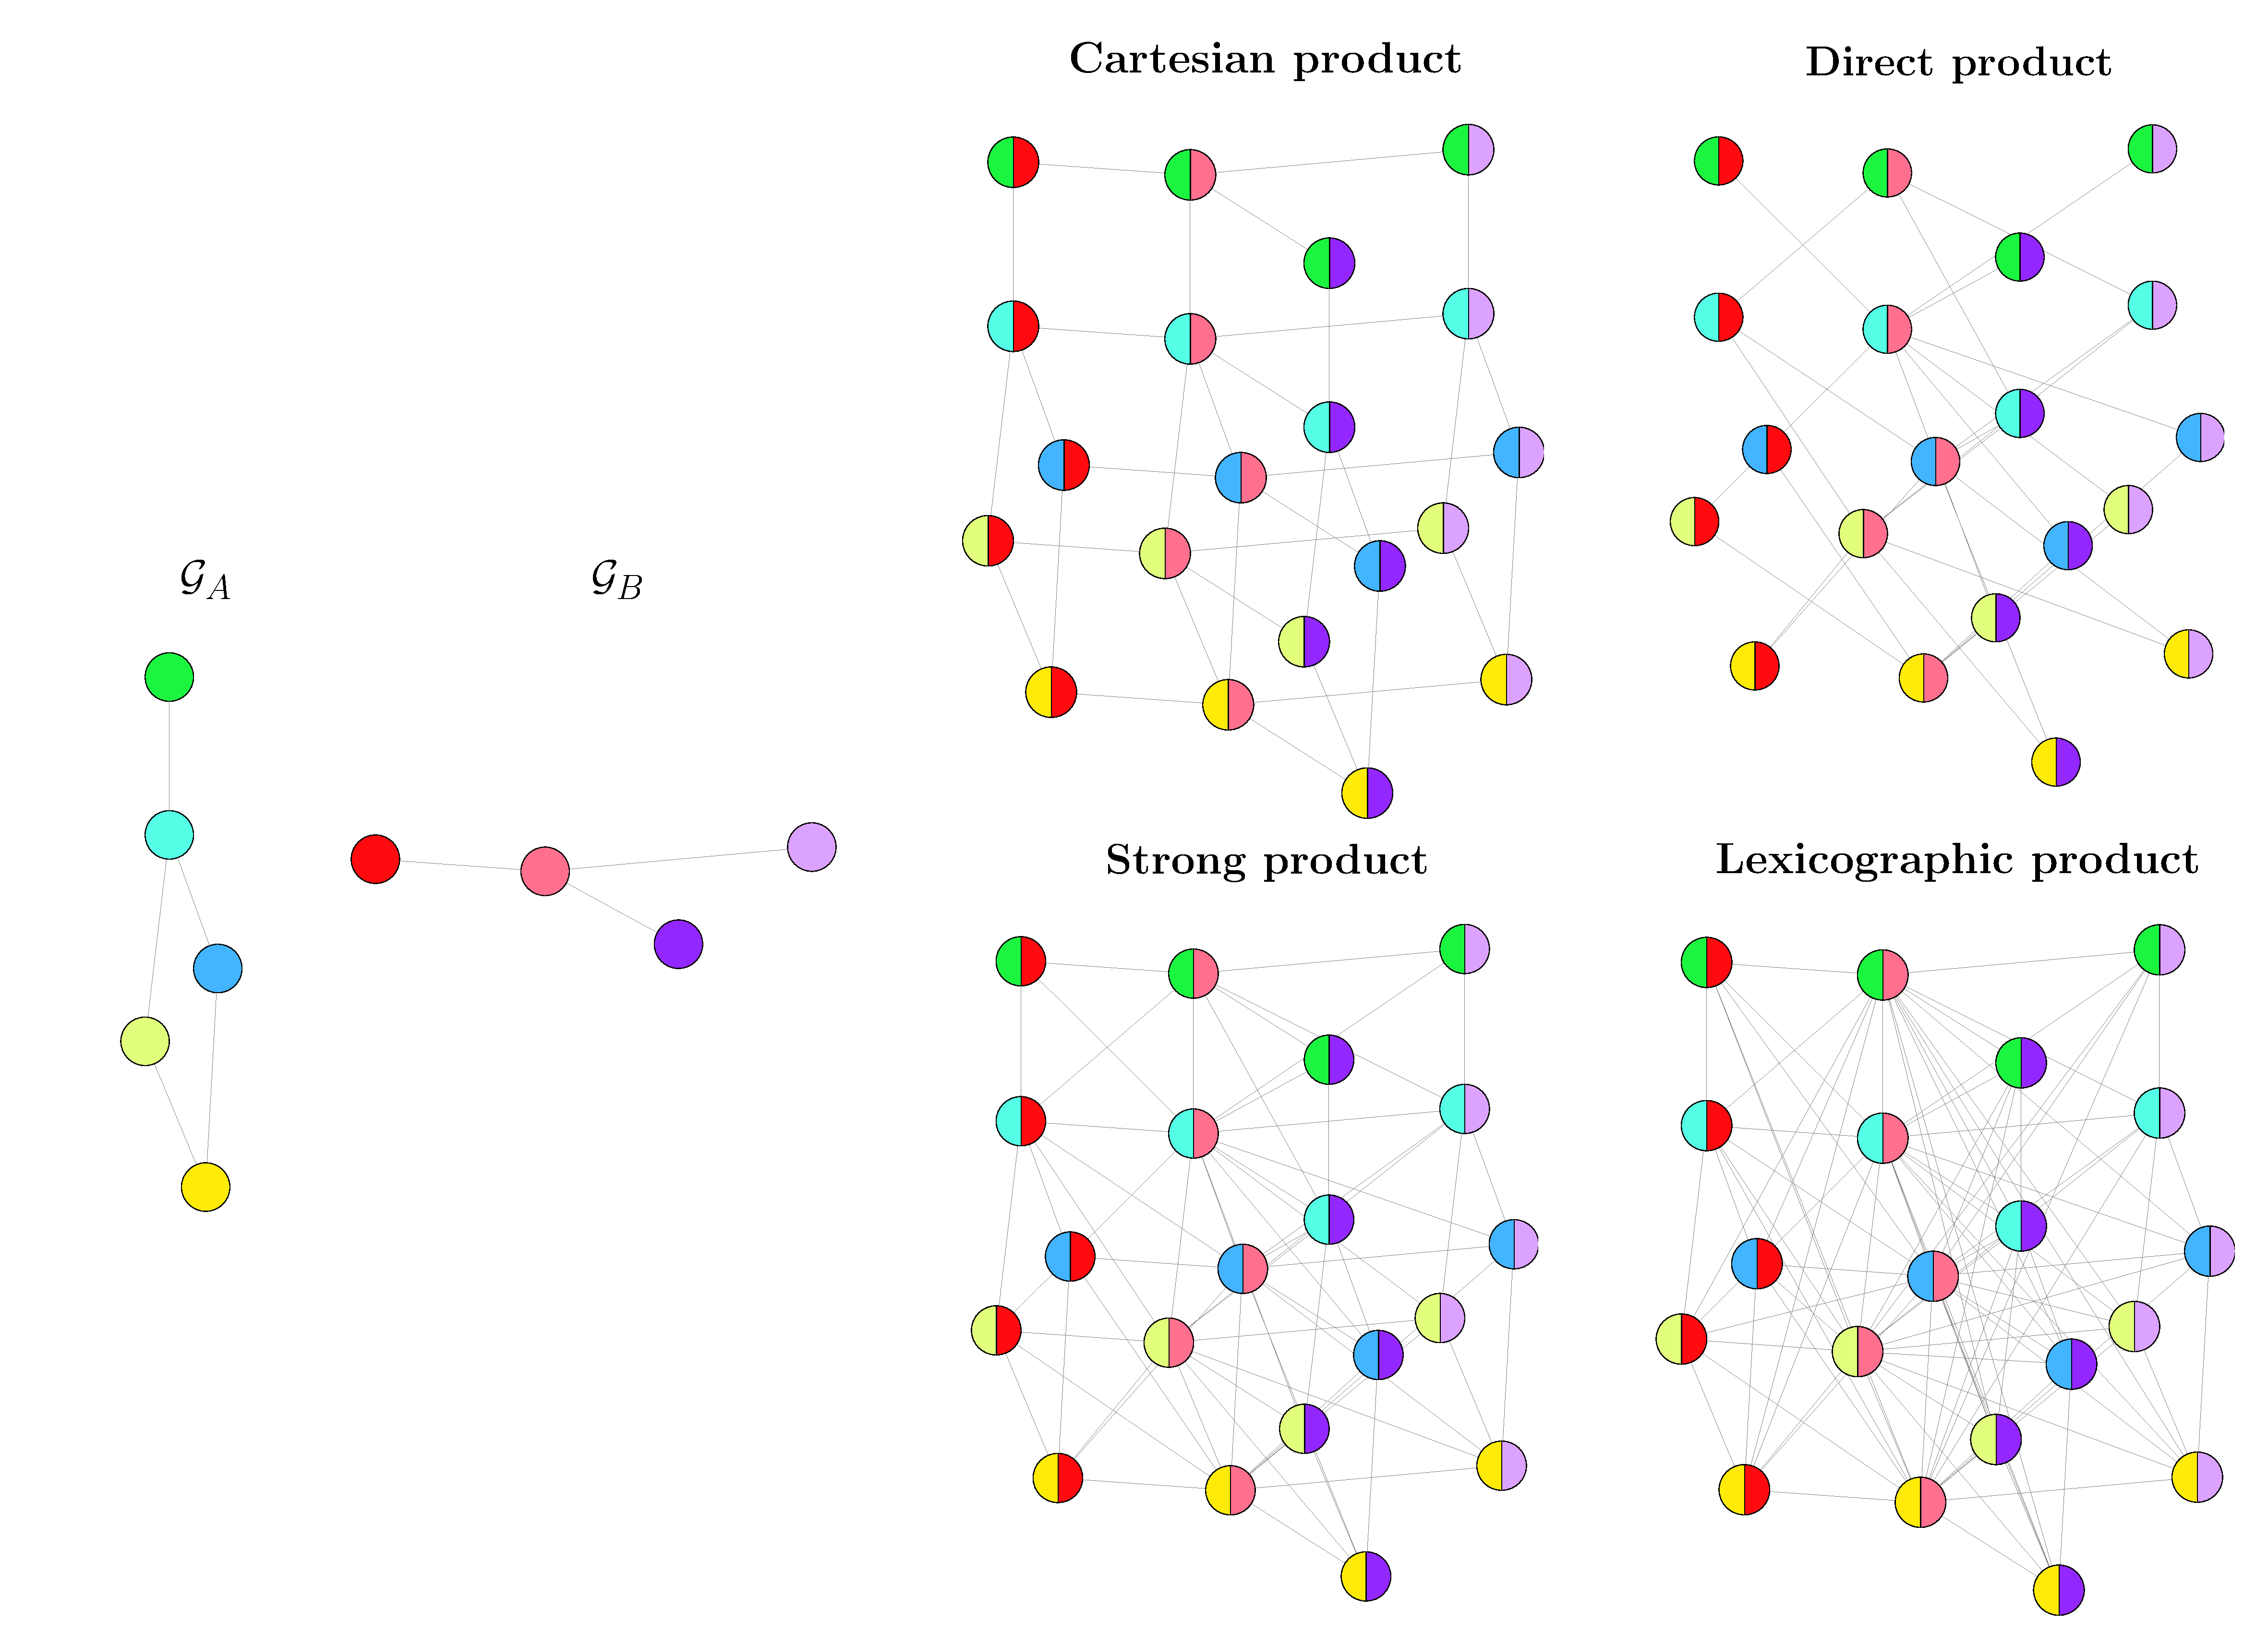
\includegraphics[width=\linewidth]{Figures/product_graphs.pdf}
    \end{center}
    \caption[Graphical depiction of the standard graph products]{A graphical depiction of the four standard graph products}
    \label{fig:graph_products}
\end{figure}

% choice of product effect the sparsity or A/cardinality of V

% What is the natural 256 ordering in terms of sparsity

% make small example in terms of vertex order

Given these definitions, it may seem that all the standard graph products are non-commutative in the sense that $\A_A \oplus \A_B  \neq \A_B \oplus \A_A $ etc. However, the graphs $\mathcal{G}_A \, \diamond \, \mathcal{G}_B$ and $\mathcal{G}_B \, \diamond \, \mathcal{G}_A$ are in fact isomorphically identical in the case of the Cartesian, direct and strong products. This is not the case for the Lexicographic product \citep{Imrich2000}.

\subsection{The spectral properties of graph products}

In the field of graph signal processing, we are often concerned with analysing the properties of graphs via eigendecomposition of the graph Laplacian \citep{Mieghem2010}. In the case of product graphs, it is greatly preferable if we are able to fully describe the spectrum of $\mathcal{G}_A \diamond \mathcal{G}_B$ in terms of the spectra of $\mathcal{G}_A$ and $\mathcal{G}_B$ alone. This is because direct decomposition of a dense $\LL$ has time-complexity $O(A^3B^3)$, whereas decomposition of the factor Laplacians individually has complexity $O(A^3 + B^3)$. As the graphs under considerations become medium to large, this fact quickly makes direct decomposition of the product graph Laplacian intractable. However, in the general case, only the spectra of the Cartesian and lexicographic graph products can be described in this way \citep{Barik2018}. In the case of the direct and strong product, it is possible to estimate the spectra without performing the full decomposition (see \citep{Sayama2016}). However, in general, the full eigendecomposition of the product graph Laplacian can only be described in terms of the factor eigendecompositions when both factor graphs are regular.


Consider the eigendecompositions of $\LL_A$ and $\LL_B$.

\begin{equation}
    \LL_A = \U_A \LAM_A \U_A^\top, \aand \LL_B = \U_B \LAM_B \U_B^\top
\end{equation}

where $\U_A$ and $\U_B$ are the respective orthonormal eigenvector matrices, and $\LAM_A$ and $\LAM_B$ are the diagonal eigenvalue matrices given by

\begin{equation}
    \LAM_A = \begin{bmatrix}
        \lambda_1^{(A)}, &                 &        &                 \\
                         & \lambda_2^{(A)} &        &                 \\
                         &                 & \ddots &                 \\
                         &                 &        & \lambda_A^{(A)} \\
    \end{bmatrix}
    \aand
    \LAM_B = \begin{bmatrix}
        \lambda_1^{(B)}, &                 &        &                 \\
                         & \lambda_2^{(B)} &        &                 \\
                         &                 & \ddots &                 \\
                         &                 &        & \lambda_B^{(B)} \\
    \end{bmatrix}
\end{equation}

Given these definitions, table \ref{tab:product_graph_spectra} gives information about the spectral decomposition of the standard graph products.

% see the effect of preconditioning matrix on different graph products 

\begin{table}[h]
    \def\arraystretch{1.8}
    \centering
    \small
    \vspace{0.5cm}
    \begin{tabular}{|l|cc|}
        \hline

         & Eigenvalues
         & Eigenvectors                                                                          \\

        \hline

        Cartesian
         & $\lambda_a^{(A)} + \lambda_b^{(B)}$
         & $(\U_A)_a \otimes (\U_B)_b$                                                           \\

        Direct$^{\star}$
         & $r_A \lambda_b^{(B)} + r_B \lambda_a^{(A)} - \lambda_a^{(A)} \lambda_b^{(B)}$
         & $(\U_A)_a \otimes (\U_B)_b$                                                           \\

        Strong$^{\star}$
         & $(1+r_A) \lambda_b^{(B)} + (1+r_B) \lambda_a ^{(A)}- \lambda_a^{(A)} \lambda_b^{(B)}$
         & $(\U_A)_a \otimes (\U_B)_b$                                                           \\

        \multirow{2}{7em}{Lexicographic$^\dagger$}
         & $B \lambda_a^{(A)}$
         & $(\U_A)_a \otimes \mathbf{1}_B$                                                       \\

         & $\lambda_b^{(B)} + B \text{deg}(a)$
         & $\mathbf{e}_a \otimes (\U_B)_b$                                                       \\

        \hline
    \end{tabular}
    \vspace{0.2cm}
    \caption[Spectral decomposition of product graphs]{Eigendecomposition of the Laplacian of the standard graph products. Here, $a$ and $b$ are understood to run from 1 to $A$ and 1 to $B$ respectively. $\star$ only for $r_A$ and $r_B$-regular factor graphs. $\dagger$ note that the $b$ runs from 2 to $B$ in the lower row. }
    \vspace{0.3cm}
    \label{tab:product_graph_spectra}
\end{table}

% remark common degree locally only necessary 
% subspace concentration 


\subsection{GSP with Cartesian product graphs}

\label{sec:gsp_cpg}

While both the direct and strong products do find uses in certain applications (for example, see \citep{Kaveh2011}), they are both less common and more challenging to work with in a graph signal processing context due to their spectral properties described in the previous subsection. In practice, being limited to regular factor graphs means the majority of practical GSP applications are ruled out. The lexicographic product does not share this drawback, however it is also significantly less common than the Cartesian product in real-world applications. For this reason, in the following, we focus primarily on the Cartesian product.

Given the spectral decomposition of the Cartesian graph product stated in table \ref{tab:product_graph_spectra}, we can write the Laplacian eigendecomposition in matrix form as follows.

\begin{equation}
    \LL = \U \LAM \U^\top, \where \U = \U_A \otimes \U_B \aand \LAM = \LAM_A \oplus \LAM_B
\end{equation}

This motivates the following definitions for the Graph Fourier Transform (GFT) and its inverse (IGFT). Consider a signal defined over the nodes of a Cartesian product graph expressed as a matrix $\Y \in \R^{B \times A}$. We can perform the GFT as follows.

% when is this well-defined? 
% FFT version?
% impose statements on the properties of Y
% stationarity? 


\begin{equation}
    \label{eq:GFT_2d}
    \text{GFT}(\Y) = \mat{\big( \U_A^\top \otimes \U_B^\top \big) \, \vecc{\Y}} = \U_B^\top \Y \U_A
\end{equation}

Correspondingly, we can define the IGFT acting on a matrix of spectral components $\Z \in \R^{B \times A}$ as follows.

\begin{equation}
    \label{eq:IGFT_2d}
    \text{IGFT}(\Z) = \mat{\big( \U_A \otimes \U_B \big)\,\vecc{\Z}} = \U_B \Z \U_A^\top
\end{equation}


\note{Product graph signals: repseprentation and vectorisation}{

    It is natural to assume that signals defined on the nodes of a Cartesian product graph $\mathcal{G}_A \, \square \; \mathcal{G}_B$ could be represented by matrices (order two tensors) of shape $(A \times B)$. Since product graph operators, such as the Laplacian $\LL_A \oplus \LL_B$, act on vectors of length $AB$, we must define a consistent function to map matrix graph signals $\in \R^{A \times B}$ to vector graph signals $\in \R^{AB}$. The standard mathematical operator for this purpose is the $\vecc{\cdot}$ function, along with its reverse operator $\mat{\cdot}$. However, this is somewhat problematic since $\vecc{\cdot}$ is defined to act in \textit{column-major} order, that is

    $$
        \text{vec} \left( \begin{bmatrix}
                \Y_{(1, 1)} & \Y_{(1, 2)} & \dots  & \Y_{(1, B)} \\
                \Y_{(2, 1)} & \Y_{(2, 2)} & \dots  & \Y_{(2, B)} \\
                \vdots      & \vdots      & \ddots & \vdots      \\
                \Y_{(A, 1)} & \Y_{(A, 2)} & \dots  & \Y_{(A, B)} \\
            \end{bmatrix} \right)
        =
        \begin{bmatrix}
            \Y_{(1, 1)} \\ \Y_{(2, 1)} \\ \vdots \\ \Y_{(A-1, B)} \\ \Y_{(A, B)}
        \end{bmatrix}
    $$

    As is visible, this does not result in a lexicographic ordering of the matrix elements when the graph signal has shape $(A \times B)$. Therefore, to avoid this issue and to be consistent with standard mathematical notation, we will assume that graph signals are represented by matrices  of shape $(B \times A)$ when considering the product between two graphs $\mathcal{G}_A \, \square \, \mathcal{G}_B$. For graph signals of this shape, the first index represents traversal of the nodes in $\mathcal{G}_B$, and the second index represents traversal of the nodes in $\mathcal{G}_A$. This ensures that matrix elements are correctly mapped to vector elements when using the column-major $\vecc{\cdot}$ function.

}

Given these definitions, we can define a spectral operator (usually a low-pass filter) $\HH$ which acts on graph signals according to a spectral scaling function $g(\lambda \,; \, \beta)$ such as one of those defined in table \ref{tab:iso_filters}. As with regular non-product graphs, the action of this operator can be understood as first transforming a signal into the Laplacian frequency domain via the GFT, then scaling the spectral components according to some function, and finally transforming back into the vertex domain via the IGFT.

\begin{align}
    \label{eq:graph_filter}
    \HH & = g(\LL_A \oplus \LL_B) \notag                                                                                          \\
        & = \big( \U_A \otimes \U_B \big) \, g \big( \LAM_A \oplus \LAM_B \big) \, \big( \U_A^\top \otimes \U_B^\top \big) \notag \\
        & = \big( \U_A \otimes \U_B \big) \, \diag{\vecc{\G}} \, \big( \U_A^\top \otimes \U_B^\top \big)
\end{align}

% remark which section of the thesis the properties of G are explained

The matrix $\G \in \R^{B \times A}$, which we refer to as the spectral scaling matrix, holds the value of the scaling function applied to the sum of
pairs of eigenvalues, such that

\begin{equation}
    \label{eq:Gba}
    \G_{ba} = g\left(\lambda^{(A)}_a + \lambda^{(B)}_b; \beta\right)
\end{equation}


% remark about Cartesian product eig sum

We observe that defining the filtering operation in this manner implies that the intensity is equal across both $\mathcal{G}_A$ and $\mathcal{G}_B$. We refer to filters of this type as \textit{isotropic}. This can be further generalised by considering an \textit{anisotropic} graph filter, which offers independent control over the filter intensity in each of the two dimensions. In this case, we define $\G$ as follows.

\begin{equation}
    \label{eq:Gba2}
    \G_{ba} =  g \left(\lambda^{(A)}_a, \lambda^{(B)}_b; \, \beta_a, \beta_b\right)
\end{equation}

where now $g$ is chosen to be an anisotropic graph filter such as one of those listed in table \ref{tab:anis_filters_2d}. Note that the original parameter $\beta$ is now replaced by two parameters $\beta_a$ and $\beta_a$ which offer control over the filter intensity in each dimension. Filters of this kind appear often in image processing literature \citep{Aubert2006}, however, their use in graph signal processing is so far limited. \Cref{fig:filters} depicts an anisotropic graph filter applied to an image, which is a special case of a 2D Cartesian product graph signal.  


\begin{table}[t]
    \def\arraystretch{1.7}
    \small
    \begin{center}
        \begin{tabular}{|l|c|}
            \hline
            \textbf{Filter}   & $g(\lambda_a, \lambda_b; \,\beta_a, \beta_b)$                                            \\
            \hline
            1-hop random walk & $(1 + \beta_a \lambda_a + \beta_b \lambda_b)^{-1}$                                   \\
            \hline
            Diffusion         & $\exp(-\beta_a \lambda_a - \beta_b \lambda_b)$                                       \\
            \hline
            ReLu              & $\max (1 - \beta_a \lambda_a - \beta_b \lambda_b, 0)$                                \\
            \hline
            Sigmoid           & $2 \big( 1 + \exp(\beta_a \lambda_a + \beta_b \lambda_b)\big)^{-1}$                  \\
            \hline
            Bandlimited       & $1, \,\text{if} \; \beta_a \lambda_a + \beta_b \lambda_b\leq 1 \; \text{else} \; 0$ \\
            \hline
        \end{tabular}
    \end{center}
    \caption{Anisotropic graph filter functions in two dimensions}
    \label{tab:anis_filters_2d}
\end{table}


\begin{figure}[t]
    % \begin{center}
    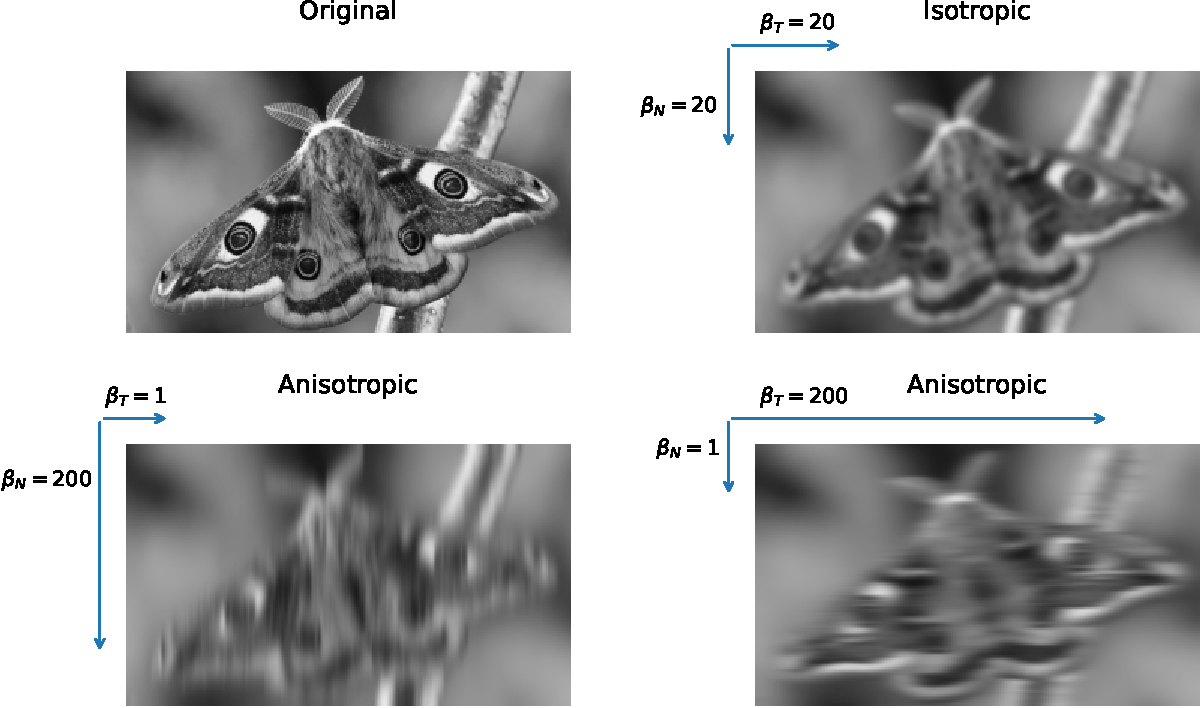
\includegraphics[width=0.9\linewidth]{Figures/filter_types_butterfly.pdf}
    % \end{center}
    \caption[A time-vertex Cartesian product graph]{A graphical depiction of a time-vertex Cartesian product graph}
    \label{fig:filters}
\end{figure}



\section{Graph Signal Reconstruction on Cartesian Product Graphs}

\label{sec:gsr_cpg}

We now turn our attention to the task of signal reconstruction on Cartesian product graphs. In the following, we will replace the factor graph labels $A$ and $B$ with $T$ and $N$ respectively. The reason for this is that one application of particular interest is graph time-series problems, where we seek to model a network of $N$ nodes across a series of $T$ discrete time points. These so called ``time-vertex'' (T-V) problems have garnered significant interest recently in the context of GSP \citep{Grassi2018, Isufi2017, Loukas2016}. T-V signals can be understood as existing on the nodes of a Cartesian product graph $\mathcal{G}_T \, \square \, \mathcal{G}_N$. In particular, we can conceptualise $T$ repeated measurements of a signal defined across the nodes of a $N$-node graph as a single measurement of a signal defined on the nodes of $\mathcal{G}_T \, \square \, \mathcal{G}_N$, where $\mathcal{G}_T$ is a simple path graph.

\vspace{1cm}


\begin{figure}[t]
    \begin{center}
        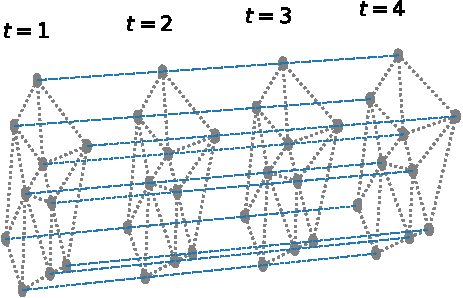
\includegraphics[width=0.5\linewidth]{Figures/T-V.pdf}
    \end{center}
    \caption[A time-vertex Cartesian product graph]{A graphical depiction of a time-vertex Cartesian product graph}
    \label{fig:TV}
\end{figure}



\note{On the Laplacian spectrum of the path graph}{
    \label{box}
    When considering time-vertex problems with uniformly spaced time intervals, $\mathcal{G}_T$ will be described by a path graph with equal weights on each edge. This special case of a graph has vertices given by $\mathcal{V}_T = \{t \in \mathbb{N} \, | \, t \leq T \}$ and edges given by $\mathcal{E}_T = \{ \, [t, t+1] \, | \, t < T \}$. The Laplacian matrix of the path graph is therefore given by

    $$
        \LL_T = \begin{bmatrix}
            1  & -1 &        &    &    \\
            -1 & 2  & -1     &    &    \\
               &    & \ddots &    &    \\
               &    & -1     & 2  & -1 \\
               &    &        & -1 & 1  \\
        \end{bmatrix}
    $$

    The eigenvalues and eigenvectors of this Laplacian are well-known and can be expressed in closed-form \citep{Jiang2012}. In particular,

    $$
        \lambda^{(T)}_t = 2 - 2 \cos \Big(  \, \frac{t - 1}{T} \pi \, \Big)
    $$

    and

    $$
        (\U_T)_{ij} = \cos \Big( \, \frac{j - 1}{T}\big(i - \frac{1}{2}\big)\pi \, \Big)
    $$

    where the columns of $\U$ are appropriately normalised such that the magnitude of each eigenvector is one. Furthermore, this implies that that the graph Fourier transform of a signal $\y \in \R^{T}$ is given by the orthogonal type-II Discrete Cosine Transform (DCT) \citep{Ahmed1974}. This is of significance, as it means we can leverage Fast Cosine Transform (FCT) algorithms \citep{Makhoul1980} which operate in a similar manner to the well-known Fast Fourier Transform (FFT) \citep{Cooley1965}. See chapter 4 of \cite{Rao1990} for an overview of FCT algorithms.

    \vspace{0.2cm}

    In particular, this reduces both of the following procedures

    \begin{equation*}
        \text{GFT}(\y) = \U^\top \y \aand \text{IGFT}(\y) = \U \y
    \end{equation*}

    from $O(T^2)$ operations to $O(T \log T)$ operations, which can be significant for large time-series problems. The figure below compares the time to compute the graph Fourier transform of a random signal using the matrix multiplication method vs the FCT implementation. In particular, we varied $T$ from 10 to 15,000 in 20 equally spaced increments, and measured the mean time to compute $\U^\top \y$ across five independent trials using both the standard matrix multiplication and the Fast Cosine Transform method. As is visible, the difference becomes extremely pronounced as $T$ grows large.

    % \begin{figure}[h]
    \begin{center}
        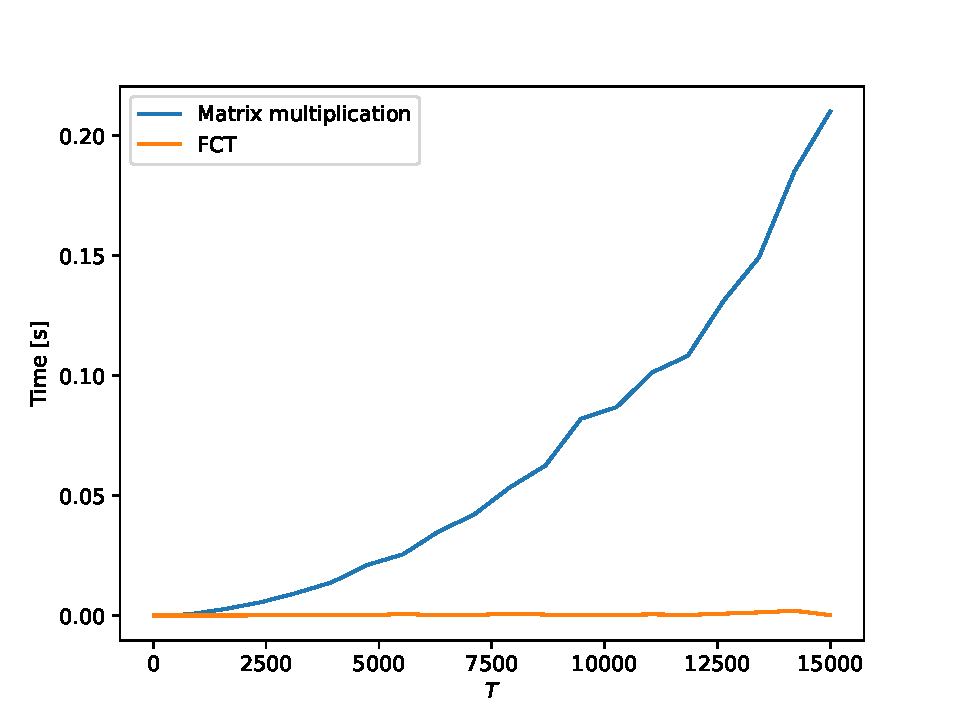
\includegraphics[width=\linewidth]{Figures/DCT.pdf}
    \end{center}
    % \caption[Run time comparison for DCT]{A graphical depiction of the four standard graph products}
    % \label{fig:DCT}
    % \end{figure} 

    % write algorithm explicitly
    % what is aliasing in this context? 
    % Nyquist for GFT? 


}



Note that, despite the observation that $\mathcal{G}_T$ is often a path graph in the context of T-V problems, the methods introduced in this section are valid for the Cartesian product between arbitrary undirected factor graphs.

\subsection{Problem statement}

\label{sec:problem_statement_2d}


The goal of Graph Signal Reconstruction (GSR) is to estimate the value of a partially observed graph signal at nodes where no data was collected. In the context of GSR on a Cartesian product graph, the available data is an observed signal $\Y \in \R^{N \times T}$ where only a partial set $\mathcal{S} = \{(n_1, t_1), (n_2, t_2), \dots \}$ of the signal elements were recorded. All other missing elements of $\Y$ are set to zero. Our model is based on the assumption that $\Y$ is a noisy partial observation of an underlying signal $\F \in \R^{N \times T}$, which is itself assumed to be smooth with respect to the graph topology.

We define the statistical model for the generation of an observation matrix $\Y$ as follows. 

\begin{equation}
    \Y = \Ss \circ \big(\F + \E \big)
\end{equation}

where $\Ss \in [0, 1]^{N \times T}$ is referred to as the sensing matrix, and has entries given by

\begin{equation}
    \Ss_{nt} = \begin{cases}
        1 & \text{if} \;\; (n, t) \in \mathcal{S} \\
        0 & \text{otherwise}
    \end{cases}
\end{equation}

The matrix $\E$ represents the model error and is assumed to have an independent normal distribution with unit variance. Therefore, the probability distribution of $\Y$ given the latent signal $\F$ is

\begin{equation}
    \label{eq:Y_given_F}
    \vecc{\Y} \, | \, \F \sim \mathcal{N}\Big(\vecc{\Ss \circ \F}, \; \diag{\vecc{\Ss}}\Big)
\end{equation}

Note that the covariance matrix $\diag{\vecc{\Ss}}$ is semi-positive definite by construction. This naturally reflects the constraint that some elements of $\Y$ are zero with probability 1. In order to estimate the latent signal $\F$, we must provide a prior distribution describing our belief about its likely profile ahead of time. In general, we expect $\F$ to be smooth with respect to the topology of the graph. This can be expressed by setting the covariance matrix in its prior to be proportional to $\HH^2$, where $\HH$ is a graph filter as defined in equation (\ref{eq:graph_filter}). For now, in the absence of any further information, we assume that the prior mean for $\F$ is zero across all elements.

\begin{equation}
    \label{eq:F_prior}
    \vecc{\F} \sim \mathcal{N}\big(\mathbf{0}, \, \gamma^{-1} \HH^2\big)
\end{equation}

Next, given an observation $\Y$, we use Bayes' rule to find the posterior distribution over $\F$. This is given by

\begin{equation}
    \pi\big(\vecc{\F} \, | \, \Y \big) = \frac{\pi\big(\vecc{\Y} \, | \, \F \big) \pi(\F) }{\pi(\Y)}.
\end{equation}

where we use the notation $\pi(\cdot)$ to denote a probability density function.

The posterior distribution for $\F$ is given by

\begin{equation}
    \label{eq:F_post}
    \vecc{\F} \, | \, \Y \sim \mathcal{N} \big(\SIG \, \vecc{\Y}, \; \SIG \big)
\end{equation}

\noindent where

\begin{equation}
    \label{eq:Sig_post}
    \SIG = \Big(\diag{\vecc{\Ss}} + \gamma  \HH^{-2}\Big)^{-1}
\end{equation}

A proof of this can be found in the appendix, theorem \ref{the:F_posterior}.



In this chapter, we are primarily interested in computing the posterior mean, which is the solution to the following linear system.

\begin{equation}
    \label{eq:lin_system}
    \vecc{\F} = \Big(\diag{\vecc{\Ss}} + \gamma  \HH^{-2}\Big)^{-1} \vecc{\Y}
\end{equation}

We return to the question of sampling from the posterior and estimating the posterior covariance directly in \cref{chap:variance}.

Two significant computational challenges arise when working with non-trivial graph signal reconstruction problems, where the number of vertices in the product graph is large. First, although the posterior mean point estimator given in \cref{eq:lin_system} has an exact closed-form solution, its evaluation requires solving an $NT \times NT$ system of equations, which is impractical for all but the smallest of problems. Second, since the eigenvalues of $\HH$ can be close to or exactly zero, $\HH^{-2}$ may be severely ill-conditioned and even undefined. This means the condition number of the coefficient matrix may not be finite, making basic iterative methods to numerically solve the linear system, such as steepest descent, slow or impossible. The models proposed in this paper aim to overcome these problems.


Since the coefficient matrix defining the system is of size $NT \times NT $, direct methods such as Gaussian elimination are assumed to be out of the question. In such cases, one often resorts to one of three possible solution approaches: stationary iterative methods; Krylov methods; and multigrid methods. Each are part of the family of iterative methods which are most commonly found in applications of sparse matrices, such as finite element methods \citep{Brenner2008}. In the following, we propose a stationary iterative method and a Krylov method and compare their relative behaviour. In both cases, we show that each step of the iterative process can be completed in $O(N^2T + NT^2)$ operations, making a solution feasible for relatively large graph problems. First, we present each of the methods in isolation. Then, the convergence behaviour of each is derived theoretically and verified numerically.


\subsection{A stationary iterative method}

\label{sec:SIM}

In this section, we demonstrate a technique for obtaining the posterior mean by adopting a classic approach to solving linear systems, known as \textit{matrix splitting}, which sits within the family of Stationary Iterative Methods (SIMs) \citep{Saad2003}. The general splitting strategy is to break the coefficient matrix into the form $\M - \N$, such that 


\begin{equation}
    \vecc{\F} = (\M - \N)^{-1} \vecc{\Y}
\end{equation}

By noting that

\begin{align}
    \M \vecc{\F} &= \N \vecc{\F} + \vecc{\Y} \\
    \vecc{\F} &= \M^{-1}\N \vecc{\F} + \M^{-1} \vecc{\Y}
\end{align}

we devise an iterative scheme given by 

\begin{equation}
    \label{eq:sim_update}
    \vecc{\F_{k+1}} = \M^{-1}\N \vecc{\F_{k}} + \M^{-1} \vecc{\Y}
\end{equation}


When $\M$ is a simple matrix that is easy to invert, this update function can be vastly more efficient to compute. Common approaches to finding a suitable value for $\M$ and $\N$ include the Jacobi, Gauss-Seidel and successive over-relaxation methods, each of which represent a different strategy for splitting the coefficient matrix \citep{Saad2003}. However, whilst these techniques are well-studied, they are not appropriate for use in the case of graph signal reconstruction. This is because, for each of these methods, the coefficient matrix is split according to its diagonal and off-diagonal elements in some way. Consequently, this would require the evaluation of $\HH^{-2}$ directly which, as we have discussed, may be large, severely ill-conditioned and possibly ill-defined. 


Instead, we require a custom splitting that avoids direct evaluation of $\HH^{-2}$, and allows the right hand side of \cref{eq:sim_update} to be computed efficiently. The main contribution of this subsection is the identification of appropriate values for $\M$ and $\N$, and an investigation of the consequences of that choice. 

In the folowing, we set 

\begin{equation}
    \M = \gamma \HH^{-2} + \I_{NT}, \aand \N = \diag{\vecc{\Ss'}}.
\end{equation}

where $\Ss'$ is the binary matrix representing the complement of the set of selected nodes, i.e.

\begin{equation}
    \label{eq:S_}
    \Ss'_{nt} = \begin{cases}
        1 & \text{if} \;\; (n, t) \notin \mathcal{S} \\
        0 & \text{otherwise}
    \end{cases}
\end{equation}

In this way, the update equation is given by 

\begin{equation}
    \label{eq:sim_update2}
    \vecc{\F_{k+1}} = \big(\gamma \HH^{-2} + \I \, \big)^{-1}  \diag{\vecc{\Ss'}} \vecc{\F_{k}} + \big(\gamma \HH^{-2} + \I \, \big)^{-1} \vecc{\Y}
\end{equation}



Note that this splitting is valid since $\big(\gamma\HH^{-2} + \I \, \big)^{-1}$ is guaranteed to exist. It can also be readily computed as we already have the eigendecomposition of $\HH$. Noting the decomposed definition of $\HH$ given in \cref{eq:graph_filter}, this can be written as

\begin{align}
    \label{eq:inv}
    \M^{-1} & = \Big( \gamma \HH^{-2} + \I \, \Big)^{-1} \notag \\
            & = \Big( \gamma \big(\U_T \otimes \U_N\big)\, \diag{\vecc{\G}}^{-2}\,  \big(\U_T^\top \otimes \U_N^\top\big)  + \I \, \Big)^{-1} \notag   \\
            & = \big(\U_T \otimes \U_N\big)\, \Big( \gamma \, \diag{\vecc{\G}}^{-2}\,    + \I \, \Big)^{-1} \big(\U_T^\top \otimes \U_N^\top\big) \notag \\
            & = \big(\U_T \otimes \U_N\big)\, \diag{\vecc{\J}}\,  \big(\U_T^\top \otimes \U_N^\top\big)
\end{align}

\noindent where $\J \in \R^{N \times T}$ has elements defined by

\begin{equation}
    \label{eq:Jnt}
    \J_{nt} = \frac{\G_{nt}^2}{\G_{nt}^2 + \gamma}.
\end{equation}

Note that the update formula can be computed with $O(N^2T + NT^2)$ complexity at each step.  


\begin{align}
    \label{eq:update3}
    \F_{k+1} & = \U_N \, \big( \J  \circ \big( \U_N^\top \, (\Ss' \circ \F_{k})\, \U_T \big) \big) \, \U_T^\top + \F_0 \\
    \label{eq:update4}
    \text{with} \quad\quad\quad \F_0 & = \U_N \, \big( \J  \circ \big( \U_N^\top \, \Y \, \U_T \big) \big) \, \U_T^\top 
\end{align}


Furthermore, this is reduced to $O(N^2T + NT \log T)$ in the case of T-V problems, and to $O\big(NT \log NT \big)$ for data residing on a grid (see \cref{box}). 


It is well-know that a given splitting will be convergent if the largest eigenvalue $\lambda_{\text{max}}$ of the matrix $\M^{-1}\N$ has an absolute value of less than one. This attribute, $\rho = |\lambda_{\text{max}}|$, is known as the spectral radius. 

Whilst the spectral radius of $\M^{-1}\N$ cannot be computed directly, we can derive an upper bound based on the properties of $\M$ and $\N$ individually. 

Consider the spectral radius of $\M^{-1}$. By directly inspecting \cref{eq:inv}, it is clear that $\rho(\M^{-1})$ will be the maximum entry in the matrix $\J$ since $\M^{-1}$ is already diagonalised in the basis $\U_T \otimes \U_N$. Consider now the definition of $\J$ given in \cref{eq:Jnt}. By definition, $g(\cdot)$ has a maximum value of one on the non-negative reals, achieved when its argument is zero. Since the graph Laplacian is guaranteed to have at least one zero eigenvalue, the maximum entry in the matrix $\J$, and therefore the spectral radius of $\M^{-1}$, is surely given by

\begin{equation}
    \rho(\M^{-1}) = \frac{1}{1 + \gamma}
\end{equation}

Next, consider the spectral radius of $\N$. This can be extracted directly as 1, since it is a diagonal binary matrix. Since both $\M^{-1}$ and $\N$ are positive semi-definite, we can apply the theorem

\begin{equation}
    \label{eq:psd}
    \rho(\A\B) \leq \rho(\A) \, \rho(\B)
\end{equation}

\citep{Bhatia1997}. Therefore, the spectral radius of $\M^{-1}\N$ is guaranteed to be less than or equal to $1 / (1 + \gamma)$.  Since $\gamma$ is strictly positive, this is less than one and, as such, convergence is guaranteed. We return to the question of convergence more thoroughly in \cref{sec:SIM_convergence}. 

Finally, the update formulas given in \cref{eq:update3,eq:update4} can be written equivalently as 

\begin{align}
    \Delta \F_0     & = \U_N \, \big( \J  \circ \big( \U_N^\top \, \Y \, \U_T \big) \big) \, \U_T^\top  \\
    \Delta \F_{k+1} & = \U_N \, \big( \J  \circ \big( \U_N^\top \, (\Ss' \circ \Delta \F_{k})\, \U_T \big) \big) \, \U_T^\top
\end{align}

In this form, the iterations can be easily terminated when $|\Delta \F_{k}|$ is sufficiently small. The complete procedure is given in algorithm \hyperlink{al:SIM}{\textbf{1}}.

\begin{algorithm}[t]
    \hypertarget{al:SIM}{}
    \caption{Stationary iterative method with matrix splitting}
    \begin{algorithmic}
        \vspace{0.05cm}
        \Require{Observation matrix $\Y \in \R^{N \times T}$}
        \vspace{0.05cm}
        \Require{Sensing matrix $\Ss \in [0, 1]^{N \times T}$}
        \vspace{0.05cm}
        \Require{Space-like graph Laplacian $\LL_N \in \R^{N \times N}$}
        \vspace{0.05cm}
        \Require{Time-like graph Laplacian $\LL_T \in \R^{T \times T}$}
        \vspace{0.05cm}
        \Require{Regularisation parameter $\gamma \in \R^{+}$}
        \vspace{0.05cm}
        \Require{Graph filter function $g(\, \cdot\, \,; \betaa \in \R^{2})$}
        \vspace{0.15cm}
        \State{Decompose $\LL_N$ into $\U_N \LAM_L \U_N^\top$ and $\LL_T$ into $\U_T \LAM_T \U_T^\top$}
        \vspace{0.15cm}
        \State{Compute $\G \in \R^{N \times T}$ as $\G_{nt} = g \left(\lambda^{(A)}_a, \lambda^{(B)}_b; \, \beta_a, \beta_b\right)$ }
        \vspace{0.15cm}
        \State{Compute $\J \in \R^{N \times T}$ as $\J_{nt} = \G_{nt}^2 / (\G_{nt}^2 + \gamma)$ }
        \vspace{0.15cm}
        \State{$\Ss' \leftarrow \mathbf{1} \in \R^{N \times T} - \Ss$}
        \vspace{0.15cm}
        \State{$\Delta\F \leftarrow \U_N\big( \J \circ (\U_N^\top \Y \U_T) \big)\U_T^\top$}
        \vspace{0.15cm}
        \State{$ \F  \leftarrow \Delta\F$}
        \vspace{0.15cm}
        \While{$|\Delta\F| > \text{tol}$}
        \vspace{0.15cm}
        \State{$\Delta\F \leftarrow \U_N \Big( \J \circ \big( \U_N^\top\, (\Ss' \circ \Delta\F ) \, \U_T \big) \Big) \U_T^\top$}
        \vspace{0.15cm}
        \State{$ \F \leftarrow  \F  + \Delta\F$}
        \vspace{0.15cm}
        \EndWhile
        \vspace{0.15cm}
        \Ensure{$ \F $}
        \vspace{0.15cm}
        \label{al:SIM}
    \end{algorithmic}
\end{algorithm}

\subsection{A conjugate gradient method}

\label{sec:CGM}

The second approach we consider for computing the posterior mean is to use the Conjugate Gradient Method (CGM). First proposed in 1952, the CGM is part of the Krylov subspace family, and is perhaps the most prominent iterative algorithm for solving linear systems \citep{Hestenes1952}. In computational terms, the method only requires repeated forward multiplication of vectors by the coefficient matrix which, in the standard CGM, bust be PSD. It is therefore effective in applications where this process can be performed efficiently. 

In brief, the CGM seeks to solve the linear system $\A \x = \bb$ by minimising, at the $k$-th iteration, some measure of error in the affine space $\x_0 + \mathcal{K}_k$ where $\mathcal{K}_k$ is the $k$-th Krylov subspace given by  

$$
\mathcal{K}_k = \text{span}\big(\rr_0, \; \A \rr_0, \, ..., \, \A^{k-1} \rr_0 \big)
$$

The residual $\rr_k$ is given by 

$$
\rr_k = \bb - \A \x
$$

and the $k$-th iterate of the CGM minimises 

$$
\phi(\x) = \frac{1}{2} \x^\top \A \x  - \x^\top \bb
$$

over $\x_0 + \mathcal{K}_k$ \citep{Kelley1995}. 

The CGM works best when the coefficient matrix $\A$ has a low condition number $\kappa$ (that is, the ratio between the largest and smallest eigenvalue is small) and, as such, a preconditioning step is often necessary. The purpose of a preconditioner is to reduce $\kappa$ by solving an equivalent transformed problem. This can be achieved by right or left multiplying the linear system by a preconditioning matrix $\PHI$. However, this likely means the coefficient matrix is no longer PSD, meaning the CGM cannot be used in its basic form. (Other approaches modified for non-PSD matrices exists, e.g. the CGNE or GIMRES \citep{Elman1982, Saad1986}). A preconditioner can also multiply the coefficient matrix on the right by a preconditioner $\PHI^\top$ and the left by $\PHI$. This preserves the symmetry meaning we can can continued to use the regular CGM. 

In our case, where the coefficient matrix is given by $\Big(\diag{\vecc{\Ss}} + \gamma  \HH^{-2}\Big)$, preconditioning will be essential for convergence. To see why, consider the definition of $\HH$ in equation (\ref{eq:graph_filter}). A low-pass filter function $g(\cdot)$ may be close to zero when applied to the  high-Laplacian frequency eigenvalues of the graph Laplacian, meaning elements of $\diag{\vecc{\G}}^{-2}$ may be very high. In the worst case, for example with a band-limited filter, the matrix $\HH$ will be singular, no matrix $\HH^{-2}$ will exist, and the condition number of the coefficient matrix will be, in effect, infinite. Therefore, the primary purpose of this subsection is to find a preconditioner that maintains efficient forward multiplication and is effective at reducing the condition number of the coefficient matrix.

References such as \citep{Saad2003} give a broad overview of the known approaches to finding a preconditioner. Standard examples include the Jacobi preconditioner which is given by the inverse of the coefficient matrix diagonal and is effective for diagonally dominant matrices, and the Sparse Approximate Inverse preconditioner \citep{Grote1997}. However, such preconditioners generally require direct evaluation of parts of the coefficient matrix or are computationally intensive to calculate.

In the following, we derive an effective symmetric preconditioner that allows forward multiplication of the coefficient matrix to be performed efficiently. First consider the transformed variable $\Z$, related to $\F$ in the following way.

\begin{equation}
    \label{eq:Z_transform}
    \F = \U_N \, (\G \circ \Z) \, \U_T^\top
\end{equation}

Here, $\Z$ can be interpreted as set of Laplacian frequency coefficients, which are subsequently scaled according to the graph filter function, and then reverse Fourier transformed back into the node domain. Matrices $\Z$ which are distributed according to a spherically symmetric distribution, result in signals $\F$ which are smooth with respect to the graph topology. Since this transform filters out the problematic high-Laplacian frequency Fourier components, the system defined by this transformed variable $\Z$ is naturally far better conditioned.

By substituting this expression for $\F$ back into the likelihood in equation (\ref{eq:Y_given_F}), and the prior of equation (\ref{eq:F_prior}), one can derive a new expression for the posterior mean of $\Z$. This is done explicitly in \cref{the:Z_transform_bayes}. The end result is that the new linear system for the transformed variable $\Z$ is given by


\begin{equation}
    \label{eq:Z_post}
    \vecc{\Z} = \big( \C + \gamma \I_T \otimes \I_N \big) ^{-1} \vecc{\G \circ (\U_N^\top \Y \U_T)}
\end{equation}

\noindent where $\C$ is the symmetric PSD matrix


\begin{equation}
    \label{eq:Q}
    \C = \D_{\G} \, \big(\U_T^\top \otimes \U_N^\top \big)\, \D_{\Ss} \, \big(\U_T \otimes \U_N \big) \,\D_{\G}
\end{equation}

\noindent where we have abbreviated $\diag{\vecc{\G}}$ and $\diag{\vecc{\Ss}}$ as $\D_{\G}$ and $\D_{\Ss}$ respectively. Note that the conditioning of the coefficient matrix $\C + \gamma \I$ is greatly improved from the untransformed problem, as we will discuss in greater detail in \cref{sec:convergence}. Note also that multiplication of a vector $\vecc{\RR}$ by the coefficient matrix can be computed efficiently as 

$$
\mat{\big(\C + \gamma \I \big)\vecc{\RR}} = \gamma \RR + \G \circ \Bigg(\U_N^\top \Big( \Ss \circ \big(\U_N (\G \circ \RR) \U_T^\top \big) \Big) \U_T\Bigg) 
$$

This has $O(N^2T + NT^2)$ complexity at each step which may be  reduced to $O(N^2T + NT \log T)$ in the case of T-V problems, and to $O\big(NT \log NT \big)$ for data residing on a grid (see \cref{box}). 

The linear system defined \cref{eq:Z_post} can be understood as a two-sided symmetrically preconditioned version of the original linear system given in \cref{eq:lin_system}. In particular, the new expression can be constructed by modifying the original system in the following way.

\begin{equation}
    \Big(\PHI^\top  \big(\D_{\Ss} + \gamma  \HH^{-2}\big) \, \PHI  \Big) \Big(\PHI^{-1}\, \vecc{ \F } \Big) = \PHI^\top \, \vecc{\Y},
\end{equation}

\noindent where

\begin{equation}
    \PHI =   \big(\U_T \otimes \U_N\big) \, \D_{\G}.
\end{equation}

Since preconditioning of the coefficient matrix on the left is achieved with $\PHI^\top$ and on the right with $\PHI$, symmetry is preserved. This ensures that one can continue to utilise algorithms tailored to work with PSD matrices. In algorithm \hyperlink{al:CGM}{\textbf{2}}, we outline a conjugate gradient method based on this new formulation. 

\begin{algorithm}[t]
    \hypertarget{al:CGM}{}
    \label{al:MVGKR}
    \caption{Conjugate gradient method with graph-spectral preconditioner}
    \begin{algorithmic}
        \vspace{0.15cm}
        \Require{Observation matrix $\Y \in \R^{N \times T}$}
        \vspace{0.05cm}
        \Require{Sensing matrix $\Ss \in [0, 1]^{N \times T}$}
        \vspace{0.05cm}
        \Require{Space-like graph Laplacian $\LL_N \in \R^{N \times N}$}
        \vspace{0.05cm}
        \Require{Time-like graph Laplacian $\LL_T \in \R^{T \times T}$}
        \vspace{0.05cm}
        \Require{Regularisation parameter $\gamma \in \R$}
        \vspace{0.05cm}
        \Require{Graph filter function $g(\, \cdot\, \,; \betaa)$}
        \vspace{0.25cm}
        \State{Decompose $\LL_N$ into $\U_N \LAM_L \U_N^\top$ and $\LL_T$ into $\U_T \LAM_T \U_T^\top$}
        \vspace{0.15cm}
        \State{Compute $\G \in \R^{N \times T}$ as $\G_{nt} = g \left(\lambda^{(A)}_a, \lambda^{(B)}_b; \, \beta_a, \beta_b\right)$ }
        \vspace{0.15cm}
        \State{Initialise $\Z \in \R^{N \times T}$ randomly}
        \vspace{0.15cm}
        \State{$\RR \leftarrow \G \circ (\U_N^\top \Y \U_T) - \gamma \Z - \G \circ \Big( \, \U_N^\top \big(\Ss \circ (\U_N \, (\G \circ \Z) \, \U_T^\top) \big)  \, \U_T\Big)$}
        \vspace{0.15cm}
        \State{$\D \leftarrow \RR$}
        \vspace{0.15cm}
        \While{$|\Delta\RR| > \text{tol}$}
        \vspace{0.15cm}
        \State{$\A_D \leftarrow \gamma \D + \G \circ \Big( \, \U_N^\top \big(\Ss \circ (\U_N \, (\G \circ \D) \, \U_T^\top) \big)\, \U_T\Big) $}
        \vspace{0.15cm}
        \State{$\alpha \leftarrow  \tr{\RR^\top \RR} \, / \, \tr{\RR^\top \A_D \RR}$}
        \vspace{0.15cm}
        \State{$\Z \leftarrow  \Z + \alpha \D $}
        \vspace{0.15cm}
        \State{$\RR \leftarrow  \RR - \alpha \A_D $}
        \vspace{0.15cm}
        \State{$\delta \leftarrow \tr{\RR^\top \RR} \, / \, \tr{(\RR + \alpha \A_D)^\top (\RR + \alpha \A_D)}$}
        \vspace{0.15cm}
        \State{$\D \leftarrow  \RR + \delta \D $}
        \vspace{0.15cm}
        \EndWhile
        \vspace{0.25cm}
        \Ensure{$\U_N \, (\G \circ \Z) \, \U_T^\top$}
        \vspace{0.15cm}
    \end{algorithmic}
\end{algorithm}

\subsection{Verifying basic properties}

In this subsection, we seek to verify several basic properties of the CGM and SIM. First, we want to show that both methods converge to the same prediction for the smooth underlying signal $\F$ an check that the solution is 


\begin{figure}[t]
    \hypertarget{butterflies}{}
    \label{fig:butterflies}
    \begin{center}
        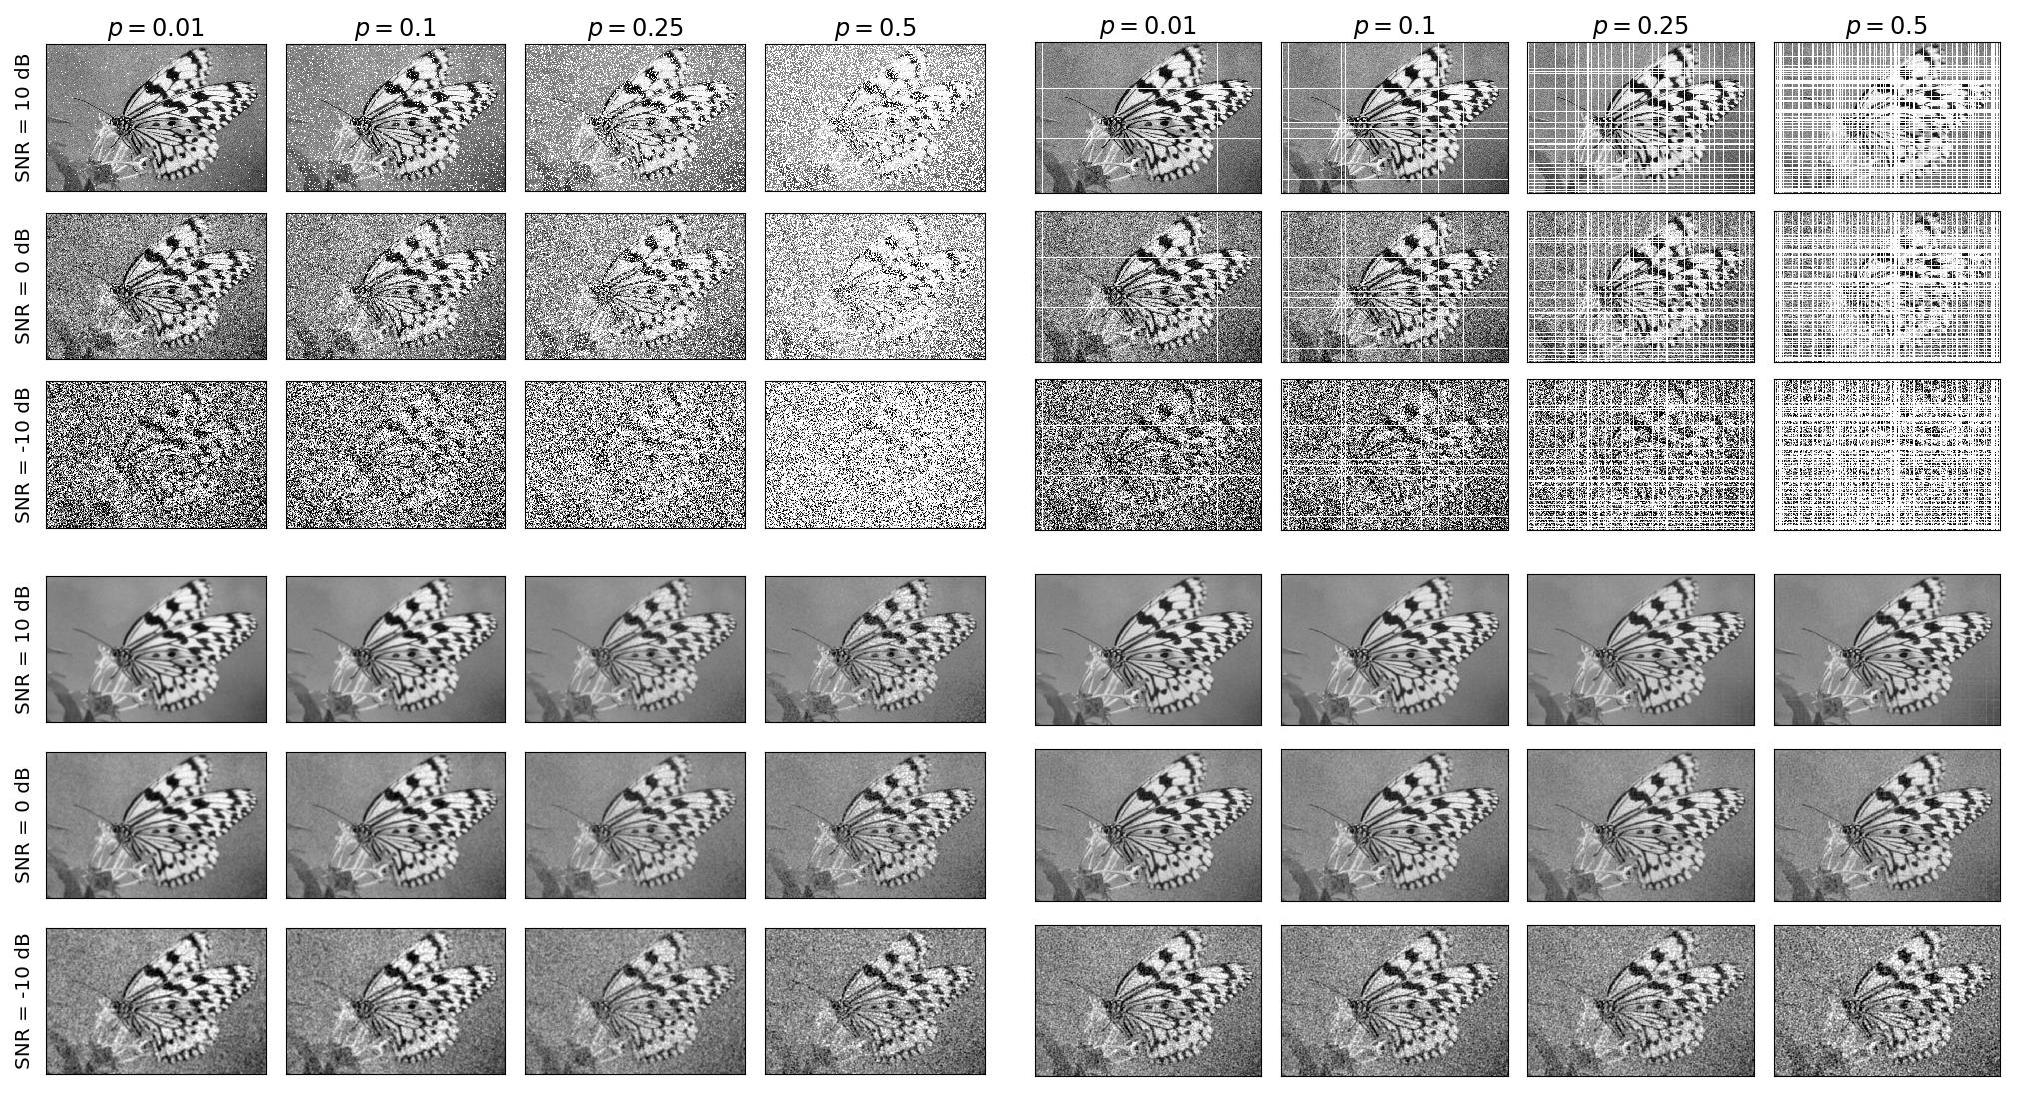
\includegraphics[width=0.95\linewidth]{Figures/butterflies.jpg}
        % \includegraphics[width=0.9\linewidth]{images/outputs.jpg}
    \end{center}
    \caption{\small{The output from the first experiment is depicted. In the top left quadrant, the input images are shown across a range of noise levels and missing pixel percentages, with missing pixels chosen uniformly at random. Below that, in the lower left quadrant, the corresponding reconstructed images are shown. The right half of the plot is the same, except here entire columns and rows of pixels are removed at random.}}
\end{figure}


\section{Convergence properties}

\label{sec:convergence}


In this section, we take a closer look at the convergence properties of both the SIM and the CGM. As we will show, the method with the best convergence rate depends on the value of the hyperparameters $\beta$, which describes the strength of the graph filter, $\gamma$, which determines the regularisation strength, and $m=|\mathcal{S}'|/NT$, which is the fraction of values that are missing from the original graph signal. For both methods, we provide bounds on the convergence rate and show how each of these three parameters can be expected to effect convergence in practice. 

We begin first with a brief review the generic convergence properties of the SIM and CGM. Next, we analyse their behaviour in the specific case of graph signal reconstruction as described in our model. We demonstrate that, for both models, the convergence rate is bounded by two edge cases; one in the limit of a weak graph filter and the other in the limit of a strong graph filter. Furthermore we show that in the weak filter limit, where $\beta \rightarrow 0$, the CGM has better convergence behaviour. On the other hand, in the strong filter limit where $\beta \rightarrow \infty$, the SIM has better convergence behaviour. We also provide intuition for selecting a method for intermediate values of $\beta$. 


\subsection{Convergence of the SIM}
\label{sec:SIM_convergence}

In the SIM, we have that 

\begin{equation}
    \label{eq:SIM_F_true}
\M \vecc{\F} =  \N \vecc{\F} + \vecc{\Y}
\end{equation}

where $\vecc{\F}$ represents the true solution to the linear system. This leads directly to an update equation given by

\begin{equation}
    \label{eq:SIM_F_update}
\M \vecc{\F_k} = \N \vecc{\F_{k-1}} + \vecc{\Y}
\end{equation}

Subtracting \cref{eq:SIM_F_true} from \cref{eq:SIM_F_update} gives

\begin{align}
    \M \vecc{\F_k} - \M \vecc{\F} &= \N \vecc{\F_{k-1}} - \N \vecc{\F}  \notag \\
    \vecc{\E_k} &= \M^{-1} \N \vecc{\E_{k-1}} \notag \\
     &= \big( \M^{-1} \N \big)^{k} \vecc{\E_{0}}
\end{align}

where we denote the error at the $k$-th iteration as $\vecc{\E_k} = \vecc{\F_k} - \vecc{\F}$. From this it is clear to see that convergence will be achieved so long as the spectral radius $\rho(\M^{-1}\N)$ is less than one. If this condition holds then,

\begin{equation}
    \lim_{k \rightarrow \infty} \vecc{\E_{k}} = \lim_{k \rightarrow \infty} (\M^{-1} \N)^{k} \, \vecc{\E_0} = \mathbf{0} .
\end{equation}

In general, the number of iterations required to achieve some specified reduction in the magnitude of the error is proportional to one over the logarithm of the spectral radius \citep{Demmel1997}. Therefore, given that 

$$
\M = \big(\U \D_\J \U^\top\big)^{-1}, \aand \N = \D_{\Ss'}
$$

where we use the shorthands

$$
\U = \U_T \otimes \U_N, \quad \D_\J = \diag{\vecc{\J}}, \aand \D_{\Ss'} = \diag{\vecc{\Ss'}}. 
$$



the complexity of the SIM in our context follows


\begin{equation}
    \label{eq:n_SIM}
    n_{\text{SIM}} \propto  -\frac{1}{\log\rho\left(\U \D_\J \U^\top \D_{\Ss'} \right)}
\end{equation}

The matrix $\J$ [see \cref{eq:Jnt}] has entries that depend on both the the regularisation parameter $\gamma$ and the spectral scaling matrix $\G$ [see \cref{eq:Gba,eq:Gba2}], which is itself a function of the graph filter parameter(s) $\beta$. The matrix $\D_{\Ss'}$  has entries that depend on the structure of the missing data in the graph signal. Therefore we expect that $\rho$, and consequently the number of steps required for convergence $n_{\text{SIM}}$, may be affected by all three of these variables.  


\subsection{Convergence of the CGM}

In the conjugate gradient method, by contrast, the number of steps required to achieve some termination condition is well-known to follow $O(\sqrt{\kappa})$, where $\kappa$ is the condition number of the coefficient matrix \cite{Kelley1995}. In our case, the coefficient matrix is given in equation (\ref{eq:Z_post}) as $\C + \gamma \I$. 



Therefore, given the definition for $\C$ given in equation (\ref{eq:Q}), we expect that the number of iterations required for convergence of the CGM will scale as

\begin{equation}
    \label{eq:n_CGM}
     n_{\text{CGM}} \propto \sqrt{\kappa \left(  \, \D_\G \U^\top \D_{\Ss} \U \D_\G + \gamma \I \; \right)}
\end{equation}

Once again, this expression contains the matrix $\G$, which depends on the strength of the graph filter function parameter $\beta$, the matrix $\D_{\Ss'}$, which depends on the missingness structure, and the parameter $\gamma$. Therefore, we should expect that, in general, convergence is affected by all three of these variables. 


\subsection{Upper bound on convergence: the weak filter limit}

Consider the limiting case of a weak filter, where all spectral components are allowed to pass through unaffected. In this case, a graph filter $\HH$ [see \cref{eq:graph_filter}] applied to any graph signal $\vecc{\Y}$ returns the same signal back 

$$
\HH \vecc{\Y} = \vecc{\Y}
$$

Given the definitions of the graph filters in \cref{tab:iso_filters,tab:anis_filters_2d}, we can conceptualise this as the limit where the parameter characterising the graph filter $\beta \rightarrow 0$ (or, more generally, the limit as $\betaa \rightarrow [0, 0]$ for an anisotropic graph filter). In this limit, every element of the spectral scaling matrix $\G$ will be equal to one. Given \cref{eq:Jnt}, this further implies the every entry in the matrix $\J$ becomes $1 / (1 + \gamma)$. Therefore, 

$$
\lim_{\beta \rightarrow 0} \; \D_\G = \I, \aand \lim_{\beta \rightarrow 0} \; \D_\J = \frac{1}{1 + \gamma} \I
$$

Now consider the spectral radius of the update matrix in the SIM. Given this limiting value of $\D_\J$, this can be directly evaluated as

\begin{align}
    \lim_{\beta \rightarrow 0} \; \rho\Big(\U \D_\J \U^\top \D_{\Ss'} \Big) &= \frac{1}{1 + \gamma} \rho\Big(\U \U^\top \D_{\Ss'} \Big) \notag \\
    &= \frac{1}{1 + \gamma} \rho\Big(\D_{\Ss'} \Big) \notag \\
    &= \frac{1}{1 + \gamma} \label{eq:beta_lim_0} 
\end{align}

Next, consider the condition number $\kappa$ of the coefficient matrix in the CGM. Again, this can be directly evaluated as 


\begin{align}
    \lim_{\beta \rightarrow 0} \; \kappa \left(  \, \D_\G \U^\top \D_{\Ss} \U \D_\G + \gamma \I \; \right) &= \kappa  \left(  \, \U^\top \D_{\Ss} \U + \gamma \I \; \right) \notag \\[0.2cm]
    &= \kappa  \left(  \, \U^\top \left( \D_{\Ss} + \gamma \I \right) \U \; \right) \notag \\[0.3cm]
    &= \frac{1 + \gamma}{\gamma}
\end{align}

 Given \cref{eq:n_SIM,eq:n_CGM}, we can characterise the number of iterations required to reach some convergence criterion in the weak filter limit for the SIM and CGM respectively as

\begin{alignat}{2}
    \label{eq:n_SIM_WFL}
    \lim_{\beta \rightarrow 0} \;  n_{\text{SIM}} \, & \propto \;\;  \frac{1}{\log(1 + \gamma)} \;\; \\[0.5cm]
    \lim_{\beta \rightarrow 0} \;  n_{\text{CGM}} \, & \propto \;\;\;  \sqrt{\frac{1}{\gamma} + 1} \; 
    \label{eq:n_CGM_WFL}
\end{alignat}

Several similarities exist between these two expressions. In both cases, the fraction of unobserved values, $m$, has no effect on the convergence rate. When $\gamma$ is high, both methods converge quickly. However, they both see the number of iterations increase to infinity as $\gamma \rightarrow 0$. To characterise this more precisely, consider the Taylor expansion of each expression around $\gamma =0$.  


\begin{align}
    \lim_{\beta \rightarrow 0} \;  n_{\text{SIM}}  \;  &\propto \gamma^{-1} \, + \, \frac{1}{2} \, - \, \frac{\gamma}{12} \, + \, O(\gamma^2) \\[0.5cm]
    \lim_{\beta \rightarrow 0} \;  n_{\text{CGM}} &\propto \, \gamma^{-1/2} \, + \, \frac{\gamma^{1/2}}{2} \, + \, O\left(\gamma^{3/2}\right) 
\end{align}

The dominant behaviour for small $\gamma$ follows $O(\gamma^{-1})$ for the SIM and $O(\gamma^{-1/2})$ for the CGM. This implies that, in the limit of a weak filter, the CGM will be generally preferable, especially when $\gamma$ is small.  


\subsection{Lower bound on convergence: the strong filter limit}

Consider now the limiting case of a strong filter, where every spectral component is filtered out except the the first Laplacian frequency component $\uu_1 \propto \mathbf{1}$ (also known as the bias), with eigenvalue $\lambda_1 = 0$, which passes through the filter unaffected. Given the definitions of the graph filter functions given in \cref{tab:iso_filters,tab:anis_filters_2d}, we can associate this with the limit as $\beta \rightarrow \infty$. Here, the graph filter operates on a generic graph signal $\vecc{\Y}$ as follows. 

$$
\HH \vecc{\Y} = \frac{\sum_{n, t} \Y_{nt}}{NT} \mathbf{1}
$$


In this case, the spectral scaling matrix $\G$ has entries that are zero for all elements except (1, 1) which has the value 1. Similarly, the matrix $\J$ has the value $1 / (1 + \gamma)$ at element (1, 1) and zeros elsewhere. 


$$
\lim_{\beta \rightarrow \infty} \; \D_\G = \mathbf{\Delta}, \aand \lim_{\beta \rightarrow \infty} \; \D_\J = \frac{1}{1 + \gamma} \mathbf{\Delta}, \where     \mathbf{\Delta} = \begin{bmatrix}
    1 & 0 & 0 & \dots \\
    0 & 0 & 0 &  \\
    \vdots & & & \ddots
\end{bmatrix} 
$$

 In the case of the SIM, the spectral radius of $\M^{-1}\N$ in this limit is 

\begin{align*}
    \lim_{\beta \rightarrow \infty} \; \rho\Big(\U \D_\J \U^\top \D_{\Ss'} \Big) &= \frac{1}{1 + \gamma} \rho\Big(\U \mathbf{\Delta} \U^\top \D_{\Ss'} \Big)
\end{align*}

Note that 

\begin{equation*}
    \U \mathbf{\Delta} \U^\top = \uu_1 \uu_1^\top  = \frac{1}{NT} \OO
\end{equation*}

where $ \OO$ is a matrix of ones. Therefore the spectral radius is given by 

\begin{align*}
    \lim_{\beta \rightarrow \infty} \; \rho(\U \D_\J \U^\top \D_{\Ss'}) &= \frac{1}{NT (1 + \gamma) } \; \rho \left( \begin{bmatrix}
        \vecc{\Ss'}^\top \\ \vecc{\Ss'}^\top \\ \dots \\ \vecc{\Ss'}^\top
    \end{bmatrix} \right)
\end{align*}

Since the matrix in brackets is just the vector $\vecc{\Ss'}^\top$ repeated in every row it is surely of rank one, and therefore must have an eigenvalue of 0 with multiplicity $NT - 1$. This implies the the only non-zero eigenvalue (and therefore the spectral radius $\rho$) is given by its trace, which is $\sum \vecc{\Ss'}_i = |\mathcal{S}'|$. Denoting  $m=|\mathcal{S}'|/NT$, this can be expressed as 

\begin{equation}
    \label{eq:beta_lim_inf}
    \lim_{\beta \rightarrow \infty} \; \rho(\U \D_\J \U^\top \D_{\Ss'}) \, = \, \frac{1}{1 + \gamma} \frac{|\mathcal{S}'|}{NT} \, = \, \frac{m}{1 + \gamma}
\end{equation}

In the case of the CGM, we have that

\begin{align}
    \lim_{\beta \rightarrow \infty} & \quad \kappa \left(  \, \D_\G \U^\top \D_{\Ss} \U \D_\G + \gamma \I \; \right)  \notag \\[0.2cm]
    &= \kappa  \left(  \, \D_{\mathbf{\Delta}} \U^\top \D_{\Ss} \U \D_{\mathbf{\Delta}}  + \gamma \I \; \right) \notag \\[0.3cm]
    &= \kappa  \left(  \, 
    \begin{bmatrix} 
        \uu_1^\top \\ 
        \mathbf{0}^\top \\
        \vdots \\ 
        \mathbf{0}^\top 
    \end{bmatrix} \D_{\Ss}  \Big[ \uu_1, \, \mathbf{0}, \, \dots, \,\mathbf{0} \Big]
    + \gamma \I \; \right) \notag \\[0.2cm]
    &= \kappa  \left(  \, \frac{1}{NT}  \begin{bmatrix}
        |\mathcal{S}| & 0 & 0 & \dots \\
        0 & 0 & 0 &  \\
        \vdots & & & \ddots
    \end{bmatrix}   + \gamma \I \; \right) \notag \\[0.3cm]
    &= \frac{1 - m + \gamma}{\gamma}
\end{align}

Given \cref{eq:n_SIM,eq:n_CGM}, we can write the scaling rate for the number of iterations in the SIM and CGM respectively. 

\begin{align}
    \label{eq:n_SIM_SFL}
    \lim_{\beta \rightarrow \infty} \;  n_{\text{SIM}} \, & \propto \;\;  \frac{1}{\log(1 + \gamma) - \log m} \;\; \\[0.5cm]
    \lim_{\beta \rightarrow \infty} \;  n_{\text{CGM}} \, & \propto \;\, \sqrt{\frac{1 - m + \gamma}{\gamma}}
    \label{eq:n_CGM_SFL}
\end{align}
 

Note that, in the case of a strong filter, the number of iterations required for convergence of the CGM, $n_\text{CGM}$, still goes to infinity as $\gamma \rightarrow 0$. However, this behaviour is no longer present for $n_\text{SIM}$, which tends towards a constant value of $-1/\log m$. Taking a Taylor series expansion of both expressions about $\gamma=0$ demonstrates the asymptotic behaviour in terms of $\gamma$ more clearly. 


\begin{align}
    \lim_{\beta \rightarrow \infty} \;  n_{\text{SIM}} \, & \propto \;\;  -\frac{1}{\log m} - \frac{\gamma}{\log^2 m} + O\left(\gamma^2\right) \\[0.5cm]
    \lim_{\beta \rightarrow \infty} \;  n_{\text{CGM}} \, & \propto \, \left(\frac{\gamma}{1 - m} \right)^{-1/2} \, + \, \frac{1}{2}\left(\frac{\gamma}{1 - m}\right)^{1/2} \, + \, O\left(\gamma^{3/2}\right) 
\end{align}

In particular, at small $\gamma$, the CGM still runs with complexity proportional to $\gamma^{-1/2}$ whereas the SIM does not involve $\gamma$ to a negative power at all. This implies that, in the strong filter limit, the SIM will be preferable when $\gamma$ is small. Note that $m$ cannot scale arbitrarily close to zero or one, since it will surely be between $1/NT$ and $1 - 1/NT$. 



\subsection{Choosing a method in practice}

We have shown that the CGM will be preferable in the limit of a weak filter, when $\beta \rightarrow 0$, and that the SIM will be preferable in the limit of a strong filter, when $\beta \rightarrow \infty$. For filters that are neither asymptotically strong or weak, i.e. positive finite values of $\beta$, it is natural to ask which method can be expected to perform better. This decision will be more significant when $\gamma$ is small since, when it is large, both methods converge quickly. A visual overview of the convergence behaviour is given in \cref{fig:conv_SIM_CGM_compared}. 

\vspace{0.5cm}

\begin{figure}[hb]
    \begin{center} 
    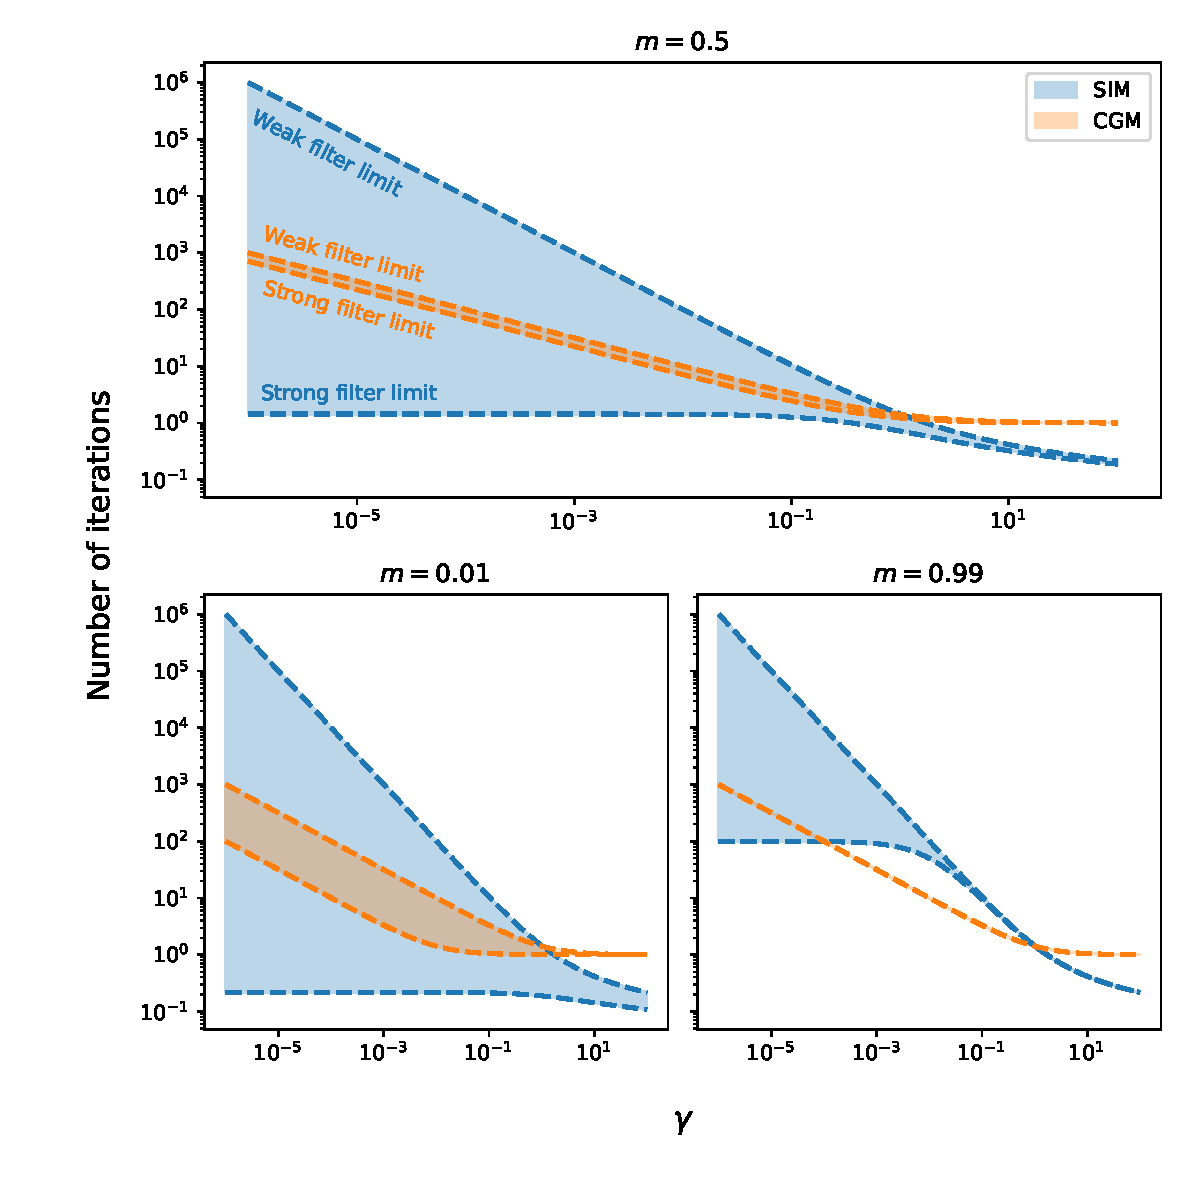
\includegraphics[width=0.85\linewidth]{Figures/conv_SIM_CGM_compared.pdf}
    \end{center}
    \caption{\small{ Here, we have plotted the functions given in \cref{eq:n_SIM_WFL,eq:n_CGM_WFL} } and \cref{eq:n_SIM_SFL,eq:n_CGM_SFL} to give a visual sense of the scaling rate of each method. Note that, since these functions are \textit{proportional} to the true number of iterations, the real values may be shifted up or down in this log-log plot.}
    \label{fig:conv_SIM_CGM_compared}
\end{figure}

In order to test the true convergence behaviour in practice, we ran a small experiment on synthetic data residing on a grid. In particular, we use a $16 \times 16$ grid of pixel data, and generated an observation matrix $\Y$ via white Gaussian noise. Next, for three different values of $m$, we chose pixels to be removed uniformly at random. We then counted the total number of iterations required to reconstruct the signal to a tolerance of $10^{-8}$ for both the SIM and the CGM, over a range of values of $\gamma$. This was done for four values of $\beta$, with a diffusion graph filter (see \cref{tab:iso_filters}). The results are shown in \cref{fig:it_gamma_plot}. 

\vspace{0.5cm}

\begin{figure}[hb]
    \begin{center} 
    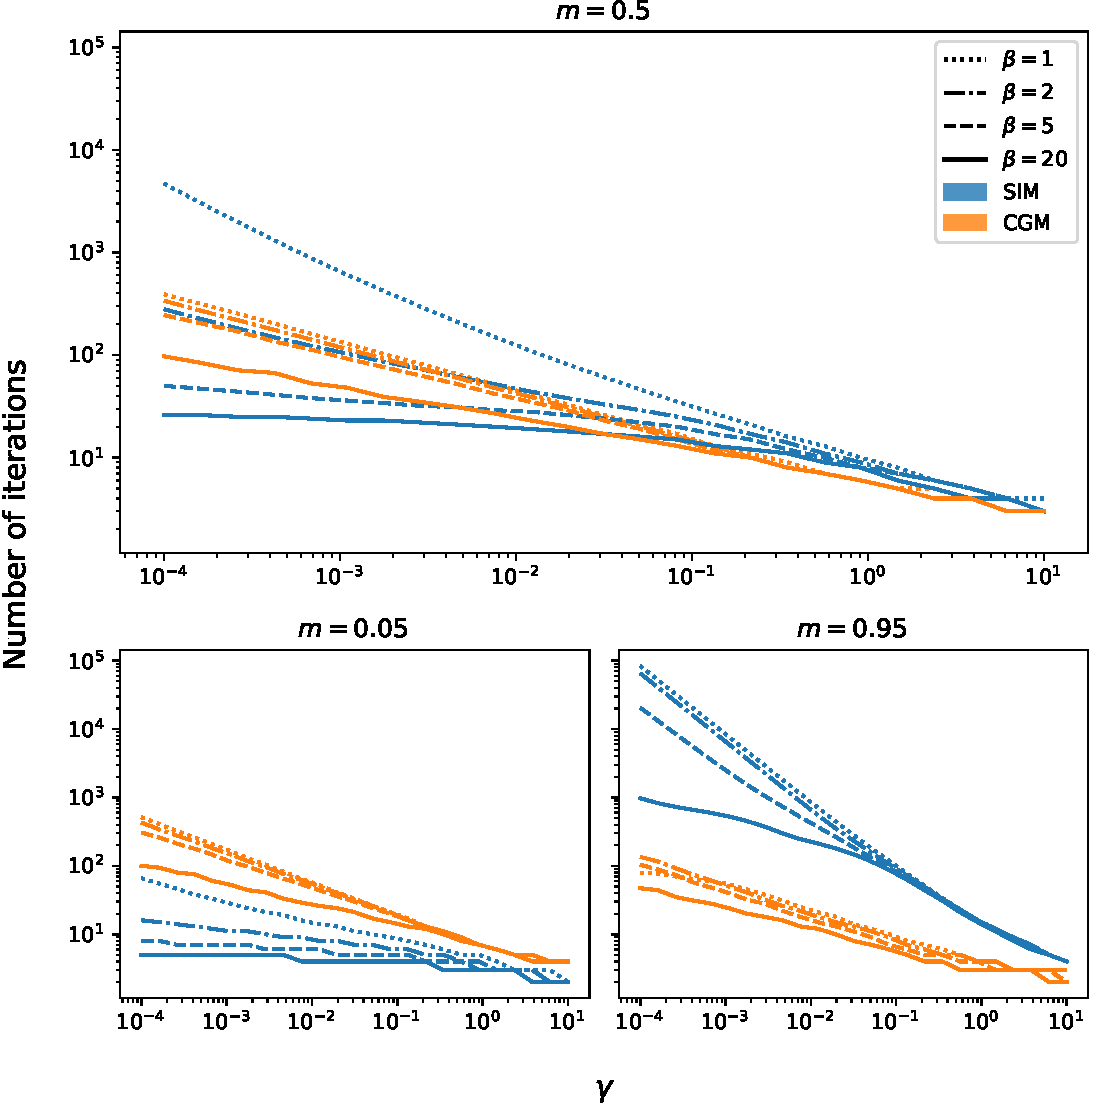
\includegraphics[width=0.9\linewidth]{Figures/experimental_its_for_conv.pdf}
    \end{center}
    \caption{\small{ The emprical number of steps required to reach some comparable convergence criteria is shown for a range of values of $\beta$ and $\gamma$ for both the SIM and CGM. Note that in all cases, $m=0.5$. }}
    \label{fig:it_gamma_plot}
\end{figure}

\vspace{0.5cm}

As is visible, the optimal choice of method will depend strongly on the choice of hyperparameters. Given these experiments, we give some ``rules-of-thumb'' for making this choice under various hyperparameter settings. This is summarised in \cref{tab:decision_SIM_CGM}. 

\definecolor{sim}{rgb}{0.12,0.47,0.71}
\definecolor{cgm}{rgb}{1,0.49,0.05}

\begin{table*}[h]
    \centering
    \footnotesize
    \def\arraystretch{1.4}
    \begin{tabular}{@{}lcccccccccccc@{}}
    \toprule
    & \multicolumn{3}{c}{Small $\gamma$} & \phantom{a} & \multicolumn{3}{c}{Medium $\gamma$} & \phantom{a} & \multicolumn{3}{c}{Large $\gamma$} \\
    \cmidrule{2-4} \cmidrule{6-8} \cmidrule{10-12}
    & S $m$   & M $m$  & L $m$ &&  S $m$   & M $m$  & L $m$ && S $m$   & M $m$  & L $m$ & \\ \midrule \rule{0pt}{0.8cm}
    S $\beta$  & \colorbox{sim!25}{SIM} & \colorbox{cgm!25}{CGM} & \colorbox{cgm!25}{CGM} && \colorbox{sim!25}{SIM} & \colorbox{cgm!25}{CGM} & \colorbox{cgm!25}{CGM} &&  \colorbox{sim!25}{SIM} & \colorbox{cgm!25}{CGM} & \colorbox{cgm!25}{CGM}    \\ \rule{0pt}{6ex}
    M $\beta$ & \colorbox{sim!25}{SIM} & \colorbox{sim!25}{SIM} & \colorbox{cgm!25}{CGM} && \colorbox{sim!25}{SIM} & \colorbox{cgm!25}{CGM} & \colorbox{cgm!25}{CGM} &&  \colorbox{sim!25}{SIM} & \colorbox{cgm!25}{CGM} & \colorbox{cgm!25}{CGM}    \\ \rule{0pt}{6ex}
    L $\beta$  & \colorbox{sim!25}{SIM} & \colorbox{sim!25}{SIM} & \colorbox{cgm!25}{CGM} && \colorbox{sim!25}{SIM} & \colorbox{sim!25}{SIM} & \colorbox{cgm!25}{CGM} &&  \colorbox{sim!25}{SIM} & \colorbox{cgm!25}{CGM} & \colorbox{cgm!25}{CGM}   \\[0.5cm] \bottomrule 
    \end{tabular}
    \caption[Rules of thumb for iterative method choice under different hyperparameter settings]{This table gives a rough rule of thumb for which iterative method should be chosen under various hyperparameter settings. S, M and L denotes small, medium and large. Note that small and large $m$ mean close to zero or one respectively, small and large $\gamma$ mean around $10^{-6}$ and around one respectively, and small and large $\beta$ mean values which cause the filter function to approach the weak and strong filter limits respectively. }
    \label{tab:decision_SIM_CGM} 
\end{table*}




 





\newpage 

\section{Conclusions}

In this chapter we have introduced a Bayesian model for the reconstruction of signals defined over the nodes of a Cartesian product graph. In particular, we show that the posterior mean of the smooth underlying signal, $\F$, is obtained by solving a linear system of size $NT \times NT$, given in \cref{eq:lin_system}. While a naive approach to computing this would have time complexity of $O(N^3T^3)$, we can utilise classic iterative methods in conjunction with the properties of the Kronecker product to solve the linear system with complexity $O(N^2T + NT^2)$ per iterative step. Furthermore, we show that this can be reduced to $O(N^2T + NT \log T)$ when considering time-vertex problems, and to $O(NT \log NT)$ when operating on a grid by making use of the Fast Cosine Transform (FCT). 

The key output of this chapter is two algorithms, namely the Stationary Iterative Method (SIM) and the Conjugate Gradient Method (CGM), tailored for the task of graph signal reconstruction. These were designed by making use of domain knowledge to produce a matrix splitting for the SIM and a preconditioner for the CGM that both guarantee bounded convergence. By analysing the spectral properties of the matrices involved in each algorithm, we provided a detailed overview of the expected convergence rate in both cases. The important results are summarised in \cref{tab:conv_SIM_CGM}, which gives a factor proportional to the number of iterations required for convergence in terms of the hyperparameters $\beta$, $\gamma$ and $m$. Given these results, we have provided some rules-of-thumb for making a choice of iterative method in practive, which is summaries in \cref{tab:decision_SIM_CGM}. This decision is of less importance when $\gamma$ is large, as both methods converge quickly in this domain, however it may be of great significance when $\gamma$ is small. 


\begin{table*}[h]
    \centering
    \def\arraystretch{1.5}
    \begin{tabular}{@{}cccccc}
    \toprule
    & \multicolumn{2}{c}{\textbf{SIM}} & \phantom{abc}& \multicolumn{2}{c}{\textbf{CGM}} \\
    \cmidrule{2-3} \cmidrule{5-6}
                               & All $\gamma$   & Small $\gamma$   &&  All $\gamma$   & Small $\gamma$ \\ \midrule \rule{0pt}{1cm}
    $\beta \rightarrow 0$      & $ \displaystyle \frac{1}{\log(1 + \gamma)}$   & $\displaystyle \gamma^{-1}$    &&    $\displaystyle \sqrt{\frac{1 + \gamma}{\gamma}}$ & $\displaystyle \gamma^{-1/2}$    \\ \rule{0pt}{6ex}
    $\beta \rightarrow \infty$ & $\displaystyle \frac{1}{\log(1 + \gamma) - \log m}$ & $\displaystyle -\frac{1}{\log m}$    &&  $\displaystyle \sqrt{\frac{1 - m + \gamma}{\gamma}}$ & $\displaystyle \left(\frac{\gamma}{1 - m} \right)^{-1/2}$ \\[0.5cm] \bottomrule 
    \end{tabular}
    \caption{The scaling behaviour of the number of steps required for convergence is shown as a function of $\gamma$ and $m$. The upper row gives the behaviour in the limit of a weak filter, and the lower row gives the behaviour in the limit of a strong filter. We also show the dominant term in the taylor expansion about $\gamma=0$ (``small $\gamma$" columns) which give a clearer picture of the asymptotic behaviour as $\gamma \rightarrow 0$. }
    \label{tab:conv_SIM_CGM} 
\end{table*}



    

% \section{Image processing experiments}

% \label{sec:im_proc_exp}


% \begin{figure}[t]
%     \hypertarget{runtime}{}
%     \label{fig:runtime}
%     \begin{center}
%         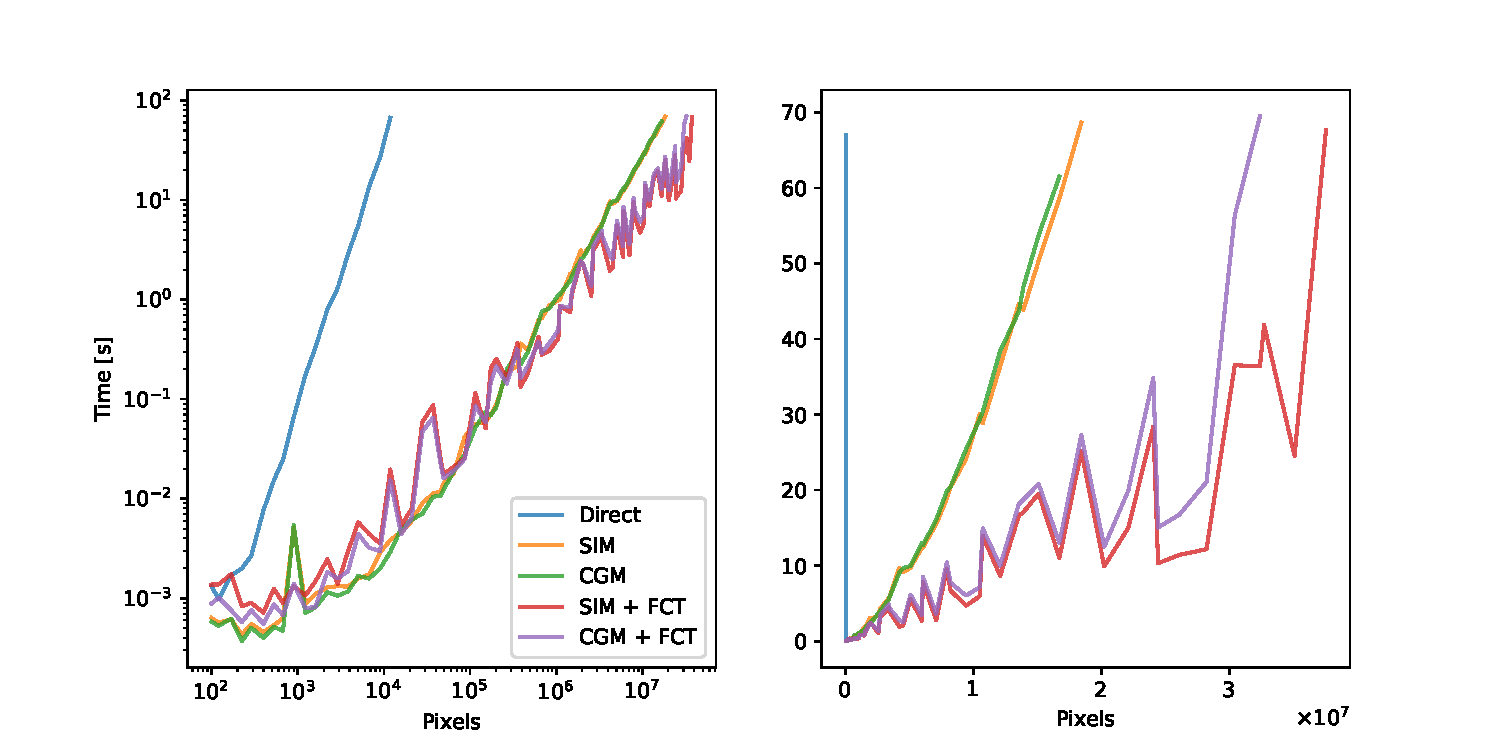
\includegraphics[width=\linewidth]{Figures/SIM_CGM_time.pdf}
%     \end{center}
%     \caption{\small{ The total runtime in seconds for the SIM and CGM compared to a naive Gaussian elimination approach is shown as a function of the total number of nodes using a quad-core Intel i7-7700HQ CPU. } }
% \end{figure}

% \begin{figure}[t]
%     \hypertarget{complexity}{}
%     \label{fig:complexity}
%     \begin{center}
%         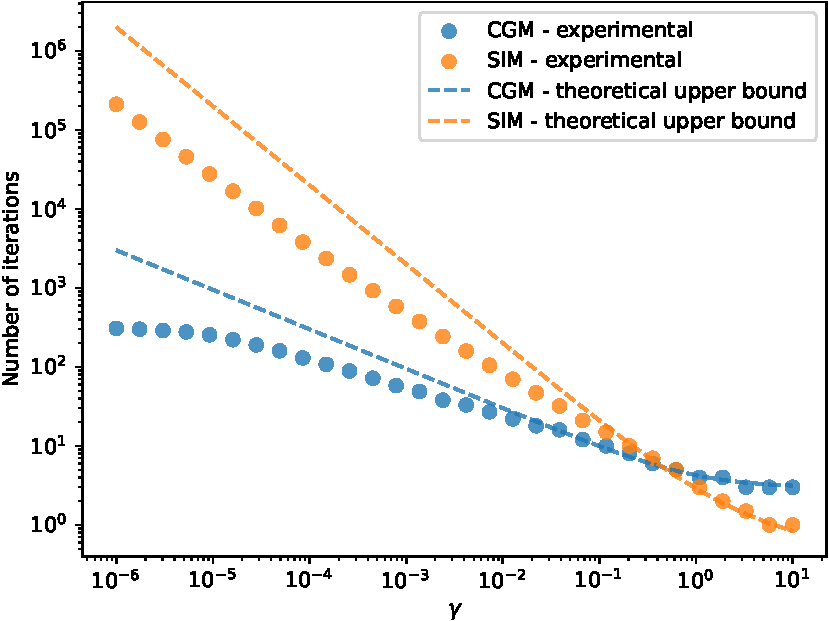
\includegraphics[width=0.7\linewidth]{Figures/complexity.pdf}
%     \end{center}
%     \caption{\small{The number of iterations required to reach a certain level of precision is shown experimentally, along with the theoretical upper bound, for the SIM and CGM} }
% \end{figure}



% % By comparing equations (\ref{eq:OSIM}) and (\ref{eq:OCGM}), we can see that the conjugate gradient method should be preferable at small $\gamma$.

% In this section, we run several small experiments to corroborate the properties of the CGM and SIM. In particular, we verify a) that both algorithms result in the same output for a given problem; b) that the runtime of the SIM and CGM increases at a significantly lower rate than naive Gaussian elimination as nodes are added; and c) that the number of iterations required for convergence as a function of $\gamma$ is less than or equal to the upper bounds derived in section \ref{sec:convergence}.

% In order to perform these checks, we use a small image denoising/reconstruction task. In particular, we use a grey-scale image of width 571 and height of 856 pixels which has been zero-centred and normalised. Note that an image can be considered a graph signal, with each pixel site representing a node connected to the other pixels immediately adjacent. Furthermore, the data itself lies on a two-dimensional lattice which is a special case of a product graph, with each sub-graph in the product being a simple chain, in this case with $N=856$ and $T=571$ respectively. Therefore, images can serve as a simple test case for checking the behaviour of product graph algorithms. Note that the purpose of this section is not to compare graph signal reconstruction to existing algorithms specialised for image denoising/reconstruction, but to examine the computational properties of GSR.

% First, we simulate a graph signal reconstruction task across a range of noise levels and missing data distributions. In particular, we add white Gaussian noise to the raw image with a Signal to Noise Ratio (SNR) of -10, 0 and 10 dB. We also remove pixels according to two rules. First, pixels are removed uniformly at random, and second, we remove entire rows and columns uniformly at random such that a fixed total percentage $p$ of the pixels is missing. We do this for $p$ equal to 0.01, 0.1, 0.25 and 0.5 giving 24 unique trials which are shown in \hyperlink{butterflies}{\textbf{figure 2}}. We find that both the SIM and the CGM converge quickly and result in identical predicted outputs, as expected. Furthermore, the statistical model seems relatively robust to noise and missing data of both types, visually performing adequately at the level of $p=0.5$ with SNR=-10dB, which is typically considered a challenging image reconstruction task.

% Next, we measured the total runtime of the SIM and the CGM as the number of nodes was increased, and compared this to a more naive approach to solving equation (\ref{eq:lin_system}) which is direct Gaussian elimination. In particular, we fixed the SNR at 0dB and the missingness to $p=0.5$, with missing pixels chosen uniformly at random, and created square images of increasing size from $10^2$ to $10^7$ total pixels. The results are shown in \hyperlink{runtime}{\textbf{figure 3}}. As is visible, the runtime of the SIM and CGM scales at a significantly slower rate that a naive approach, remaining tractable at well above $10^7$ nodes.

% Finally, we test the effect that varying the hyperparameter $\gamma$ has on the number of iterations required for convergence. To do this, we fixed the SNR at 0dB and the missingness to $p=0.5$, with missing pixels chosen uniformly at random. Next, we varied $\gamma$ in logarithmically spaced increments from $10^{-6}$ to $10^1$. For each unique value of $\gamma$, we ran both the SIM and the CGM and counted the number of steps required for each algorithm to reach a specific level of precision ($10^{-8}$ across all elements). The results are shown in \hyperlink{complexity}{\textbf{figure 4}}. We also plot the theoretical upper bound derived in the previous subsection for each method.

% As is visible, both methods converge within the bounds of their theoretical worst-case complexity. As expected, the CGM takes significantly fewer iterations than the SIM to converge at small $\gamma$. It is also visible that the CGM seems to outperform the theoretical worst-case scaling of $\gamma^{-0.5}$, converging with a rate closer to $\gamma^{-0.3}$ over the majority of the range, and even showing signs of reducing further at very small $\gamma$. The SIM on the other hand empirically converges slightly faster but close to the theoretical worst-case rate of $\gamma^{-1}$. Interestingly, the SIM converges faster than the CGM at relatively high $\gamma$, with the cross-over occurring at around $\gamma=0.5$. Although the absolute number of iterations required for convergence in this domain is low (between 1 and 10), this could still be significant for very large problems, meaning it still has some value as a solution.










